\documentclass[review]{elsarticle}

\usepackage[utf8]{inputenc}
\usepackage{amsmath,amssymb}
\usepackage{graphicx}
\usepackage{booktabs}
\usepackage{algorithm}
\usepackage{algpseudocode}
\usepackage{listings}
\usepackage{xcolor}
\usepackage{hyperref}
\usepackage{multirow}
\usepackage{tikz}
\usepackage{pgfplots}
\pgfplotsset{compat=1.18}
\usetikzlibrary{arrows.meta,positioning,shapes.geometric,fit,calc,backgrounds,decorations.pathreplacing}

\biboptions{authoryear}

\journal{Expert Systems with Applications}

% Custom colors for listings
\definecolor{codegreen}{rgb}{0,0.6,0}
\definecolor{codegray}{rgb}{0.5,0.5,0.5}
\definecolor{codepurple}{rgb}{0.58,0,0.82}
\definecolor{backcolour}{rgb}{0.95,0.95,0.92}

\lstdefinestyle{mystyle}{
    backgroundcolor=\color{backcolour},
    commentstyle=\color{codegreen},
    keywordstyle=\color{codepurple},
    numberstyle=\tiny\color{codegray},
    basicstyle=\ttfamily\footnotesize,
    breaklines=true,
    frame=single
}
\lstset{style=mystyle}

\begin{document}

\begin{frontmatter}

\title{Multi-Strategy GraphRAG for Financial Institutions: Security, Grounding, and Token Economy}

\author[inst1]{Anonymous Author\corref{cor1}}
\cortext[cor1]{Corresponding author}
\ead{anonymous@institution.edu}
\affiliation[inst1]{organization={Anonymous Institution}, country={Country}}

\begin{highlights}
\item Multi-strategy GraphRAG architecture for financial institutions
\item Formal security model with five-threat analysis for financial RAG
\item Intent-aware retrieval fusion reduces hallucination by 14 pp
\item Structured graph retrieval cuts token consumption by 70 percent
\item Open-source implementation with three financial applications
\end{highlights}

\begin{abstract}
Financial institutions increasingly deploy large language models for compliance verification, risk analysis, and audit support, yet conventional Retrieval-Augmented Generation systems fail to meet the stringent requirements of regulated environments. Standard vector-based retrieval lacks multi-hop reasoning capability, offers no formal security guarantees for multi-tenant deployments, produces insufficiently grounded responses, and incurs prohibitive token costs when processing large regulatory corpora. We propose a multi-strategy GraphRAG architecture that jointly addresses four pillars critical to financial adoption: security, hallucination reduction, token economy, and processing speed. Our system combines a domain-specific financial ontology with an ingestion pipeline that extracts knowledge graph triples via LLM-based extraction and entity resolution, and a retrieval engine that fuses three parallel strategies---graph traversal, vector similarity, and community summarization---with intent-aware weighting across six query types. We formalize a threat model for GraphRAG in regulated environments and implement defense mechanisms including tenant isolation, role-based access control, and comprehensive audit logging, mapped to LGPD, GDPR, Basel~III, and SOX requirements. Empirical evaluation across 200 regulatory questions and a 50-question financial benchmark demonstrates that the proposed system achieves 87.4\% faithfulness (versus 72.9\% for VectorRAG), 96.4\% source attribution, 70\% token reduction compared to full-document retrieval, median latency of 1.8 seconds with parallel retrieval, and 0\% cross-tenant data leakage. We validate the architecture through three financial applications: regulatory compliance, SEC filing analysis, and internal audit question answering.
\end{abstract}

\begin{keyword}
GraphRAG \sep Knowledge Graph \sep Financial NLP \sep Retrieval-Augmented Generation \sep Security \sep Hallucination Reduction \sep Token Efficiency
\end{keyword}

\end{frontmatter}

%% ============================================================
%% SECTION 1: INTRODUCTION
%% ============================================================
\section{Introduction}
\label{sec:introduction}

\subsection{Context}
\label{sec:context}

Large language models (LLMs) have rapidly transformed information processing across industries, and the financial sector is no exception. Banks, insurance companies, asset managers, and regulatory bodies are increasingly deploying LLM-based systems for a wide range of critical functions, including regulatory compliance verification, internal audit support, financial report analysis, and risk assessment \citep{pwc2024graphllm}. The appeal is clear: LLMs can process vast quantities of unstructured text---regulatory frameworks spanning hundreds of pages, SEC filings with complex cross-references, and audit reports with intricate finding hierarchies---and distill them into actionable responses for domain experts.

Retrieval-Augmented Generation (RAG) has emerged as the dominant paradigm for grounding LLM responses in authoritative document collections, mitigating the well-documented tendency of language models to hallucinate plausible but incorrect information \citep{lewis2020rag}. By retrieving relevant passages from a knowledge base before generating a response, RAG systems provide a mechanism for factual grounding that is essential in regulated environments where every claim must be traceable to its source.

The global adoption of RAG in financial services is accelerating. A recent PwC report identifies graph-enhanced LLMs as the next frontier in banking and insurance transformation, with applications spanning risk assessment, fraud detection, customer analytics, and regulatory compliance \citep{pwc2024graphllm}. Concurrently, the academic community has produced a growing body of work on RAG for financial document processing \citep{islam2023financebench, ragfinancial2025}, reflecting both the demand from practitioners and the unique challenges posed by the financial domain.

\subsection{Problem statement}
\label{sec:problem}

Despite the promise of RAG, conventional vector-based retrieval systems fail systematically in the financial context for five fundamental reasons:

\textbf{Reason 1: Multi-hop reasoning is mandatory.} Financial queries frequently require traversing chains of relationships across entities. For example, determining which subsidiaries of a given company have risk exposure to a specific country under Basel~III Pillar~2 requires navigating corporate structure hierarchies, geographic exposure mappings, and regulatory requirement chains. Vector-based retrieval returns semantically similar chunks in isolation but cannot connect these relational chains, leading to incomplete or incorrect answers \citep{han2025ragvsgraphrag}.

\textbf{Reason 2: Regulatory traceability is required by law.} Every response concerning compliance must cite specific regulatory articles. Financial regulators demand that institutions demonstrate the provenance of compliance assessments. Vector retrieval returns chunks that are semantically similar to the query but frequently from the wrong article or section, undermining the legal defensibility of the response.

\textbf{Reason 3: Hallucination is unacceptable.} In compliance and audit contexts, a hallucinated response can result in regulatory fines (e.g., up to 2\% of annual revenue under Brazil's LGPD), central bank sanctions, personal legal liability for directors, or even loss of operating licenses. The tolerance for factual inaccuracy is effectively zero in these applications.

\textbf{Reason 4: Token costs explode with financial documents.} Financial documents are characteristically long and dense. A typical SEC 10-K filing contains approximately 80,000 tokens; the Basel~III framework exceeds 200,000 tokens. Processing these documents in their entirety for every query results in prohibitive API costs. At current pricing, answering a single query against a complete 10-K filing costs approximately \$0.24 in input tokens alone, making large-scale deployment economically infeasible without structured retrieval.

\textbf{Reason 5: Multi-tenant data isolation is a regulatory requirement.} In a bank, the compliance department's QA system must not access audit department data, and vice versa. The unified vector store architecture of conventional RAG offers no mechanism for granular data isolation, creating a regulatory violation risk in multi-departmental deployments.

\subsection{Gap in the literature}
\label{sec:gap}

GraphRAG---the integration of knowledge graphs into the RAG pipeline---has emerged as a promising approach to address the limitations of vector-only retrieval. The foundational work by \citet{edge2024graphrag} demonstrated that graph-based indexing with community detection substantially improves comprehensiveness and diversity for global sensemaking queries. Subsequent work has explored GraphRAG for financial applications \citep{sarmah2024hybridrag, arun2025finreflectkg, graphcompliance2025}, token efficiency \citep{terag2025, lazygraphrag2025, polyg2025}, and security \citep{ragsecurity2025, privacyrisks2025, sag2025}.

However, no existing work addresses all four challenges simultaneously. As shown in Table~\ref{tab:comparison}, each prior contribution focuses on a subset of the requirements:

\begin{itemize}
    \item \textbf{HybridRAG} \citep{sarmah2024hybridrag} combines graph and vector retrieval for earnings call analysis but lacks a security model, community detection, and token optimization.
    \item \textbf{GraphCompliance} \citep{graphcompliance2025} achieves +4.1--7.2 percentage points in micro-F1 for GDPR compliance verification but does not address financial ontology design or token economy.
    \item \textbf{FinReflectKG} \citep{arun2025finreflectkg} provides an open-source financial knowledge graph from SEC 10-K filings but lacks a retrieval system and security model.
    \item \textbf{TERAG} \citep{terag2025} and \textbf{PolyG} \citep{polyg2025} achieve dramatic token reductions (89--97\% and 95\%, respectively) but do not address financial domain constraints or security.
    \item \textbf{Privacy-aware RAG} research \citep{ragsecurity2025, privacyrisks2025, sag2025} formalizes threat models and proposes cryptographic defenses but does not integrate these into domain-specific GraphRAG architectures.
\end{itemize}

The gap is clear: no existing system jointly provides (1)~a financial domain ontology, (2)~a formal security model for regulated multi-tenant environments, (3)~multi-strategy retrieval with intent-aware fusion, and (4)~token economy optimization---validated with a functional implementation and empirical financial applications.

\subsection{Contributions}
\label{sec:contributions}

This paper makes the following contributions:

\begin{enumerate}
    \item \textbf{Formal security model for financial GraphRAG.} We define a threat model with five attack vectors specific to GraphRAG in regulated environments, propose six defense mechanisms, and map them to four regulatory frameworks (LGPD, GDPR, Basel~III, SOX). Empirical red-team evaluation demonstrates 0\% cross-tenant data leakage and less than 5\% entity extraction attack success.

    \item \textbf{Multi-strategy retrieval with intent-aware fusion.} We propose an architecture that executes three retrieval strategies in parallel---graph traversal, vector similarity, and community summarization---and fuses their results using weights adapted to the detected query intent across six intent types. This achieves 87.4\% faithfulness, a 14.5 percentage point improvement over VectorRAG.

    \item \textbf{Token economy framework.} We quantify and optimize token consumption through structured graph retrieval, community summaries, query caching, and batch processing for indexation. The system achieves 70\% token reduction compared to full-document retrieval and 50\% indexation cost savings via Batch API processing.

    \item \textbf{Financial domain ontology.} We define a formal ontology with 10 entity types and 14 relationship types validated against regulatory documents (Basel~III, LGPD, GDPR) and financial filings (SEC 10-K/10-Q), with entity resolution supporting exact, case-insensitive, and fuzzy matching.

    \item \textbf{Open-source reference implementation and empirical evaluation.} We provide a complete implementation (Neo4j + PostgreSQL + Claude API + FastAPI) and validate it through five experiments across three financial applications: regulatory compliance QA, SEC filing analysis, and internal audit support.
\end{enumerate}

\subsection{Paper organization}
\label{sec:organization}

The remainder of this paper is organized as follows. Section~\ref{sec:related} reviews related work across four research threads: GraphRAG architectures, RAG for financial applications, security in RAG systems, and token efficiency. Section~\ref{sec:architecture} presents the system architecture, including formal notation, the ingestion pipeline, multi-strategy retrieval, and the security model. Section~\ref{sec:methodology} describes the experimental methodology, baselines, metrics, datasets, and evaluation protocol. Section~\ref{sec:results} reports experimental results across five experiments. Section~\ref{sec:applications} presents three empirical financial applications. Section~\ref{sec:discussion} discusses limitations and practical deployment considerations. Section~\ref{sec:conclusion} concludes with implications and future work.


%% ============================================================
%% SECTION 2: RELATED WORK
%% ============================================================
\section{Related work}
\label{sec:related}

We organize the related work into four research threads corresponding to the pillars of our contribution: GraphRAG architectures (Section~\ref{sec:rw-graphrag}), RAG for financial applications (Section~\ref{sec:rw-finance}), security in RAG systems (Section~\ref{sec:rw-security}), and token efficiency (Section~\ref{sec:rw-tokens}).

\subsection{GraphRAG architectures}
\label{sec:rw-graphrag}

The integration of knowledge graphs into the RAG pipeline has evolved rapidly since the foundational work of \citet{edge2024graphrag}, who proposed using LLMs to derive a knowledge graph from source documents and pre-generate community summaries using the Leiden algorithm \citep{traag2019leiden}. Their approach demonstrated substantial improvements in comprehensiveness and diversity for global sensemaking queries over corpora in the million-token range. Two comprehensive surveys formalize the GraphRAG workflow: \citet{peng2024graphrag} define a taxonomy spanning graph-based indexing, graph-guided retrieval, and graph-enhanced generation, while \citet{han2025graphragsurvey} propose a holistic framework identifying key components including query processor, retriever, organizer, generator, and data source.

Several architectural variants have since emerged. LightRAG \citep{guo2024lightrag} introduces dual-level retrieval with incremental graph updates, achieving 200ms mean response times without requiring full graph reconstruction. HippoRAG \citep{gutierrez2024hipporag} draws on neurobiological models of hippocampal memory indexing, orchestrating LLMs, knowledge graphs, and Personalized PageRank to achieve performance comparable to iterative retrieval methods while being 10--30$\times$ cheaper and 6--13$\times$ faster. SubgraphRAG \citep{li2025subgraphrag} demonstrates that extracting relevant subgraphs and reasoning over them with even smaller LLMs (Llama3.1-8B) delivers competitive and explainable results, with GPT-4o achieving state-of-the-art without fine-tuning. GRAG \citep{hu2024grag} addresses retrieval over networked documents using a divide-and-conquer strategy for optimal subgraph retrieval in linear time.

Community detection plays a central role in many GraphRAG architectures. CommunityKG-RAG \citep{chang2024communitykg} integrates community structures within knowledge graphs for fact-checking, using the Louvain algorithm to enable contextually-aware retrieval with 56.24\% accuracy using LLaMA-2 7B. More recently, \citet{corehierarchy2026} propose k-core decomposition as an alternative to Leiden-based community hierarchies, potentially offering better efficiency for large-scale knowledge graphs.

A critical perspective has emerged regarding the actual gains of GraphRAG. \citet{unbiased2025} discover that win rates for GraphRAG methods are generally lower than originally reported; for example, LightRAG's reported 66.7\% win rate against NaiveRAG drops to 39.1\% under unbiased evaluation. Similarly, \citet{whenusegraphs2025} investigate systematically when GraphRAG succeeds, noting that it frequently underperforms vanilla RAG in many real-world tasks, while excelling specifically in multi-hop reasoning scenarios. These findings underscore the importance of rigorous evaluation methodology, which we adopt in our experimental design.

\subsection{RAG for financial applications}
\label{sec:rw-finance}

The application of RAG and knowledge graphs to financial domains has attracted growing attention from both industry and academia. HybridRAG \citep{sarmah2024hybridrag}, a collaboration between BlackRock and NVIDIA, combines knowledge graph-based retrieval with vector retrieval for question answering on earnings call transcripts, demonstrating that hybrid approaches outperform either strategy in isolation. However, HybridRAG lacks community detection, security mechanisms, and token optimization.

On the knowledge graph construction side, FinReflectKG \citep{arun2025finreflectkg} provides an open-source financial knowledge graph built from SEC 10-K filings of all S\&P 100 companies, introducing a three-mode extraction pipeline (single-pass, multi-pass, reflection-agent-based) achieving 64.8\% compliance with quality rules. FinDKG \citep{li2024findkg} constructs dynamic knowledge graphs from financial news articles with 12 meta-entity types and 15 relation types, applying a GNN-based KGTransformer for temporal analysis with approximately 15\% improvement in prediction metrics. These works demonstrate the feasibility of automated financial knowledge graph construction but do not address the retrieval and generation aspects of a complete GraphRAG pipeline.

For regulatory compliance, GraphCompliance \citep{graphcompliance2025} represents regulatory texts as Policy Graphs and execution contexts as Context Graphs, achieving 4.1--7.2 percentage points improvement in micro-F1 over LLM-only and RAG baselines in 300 real-world GDPR scenarios. RAGulating Compliance \citep{jomraj2025ragulating} proposes a multi-agent framework that integrates regulatory knowledge graph triples with RAG for compliance QA. Both works demonstrate the value of graph-structured representations for regulatory text processing but do not address multi-tenant security or token economy.

FinanceBench \citep{islam2023financebench} provides a standardized evaluation framework with 10,231 questions on publicly traded companies, covering information lookup, numerical reasoning, and logical inference from SEC filings. This benchmark has become essential for evaluating RAG systems in the financial domain and informs our evaluation protocol.

Additional perspectives include the application of knowledge graphs to financial fraud detection via graph neural networks, achieving 95.4\% accuracy with hybrid LSTM-GraphSAGE models \citep{frauddetection2024}, intelligent audit systems that automate compliance checking through KG-based reasoning \citep{kgaudit2024}, and cross-jurisdictional regulatory mapping through AI-powered knowledge graphs \citep{kgfinreporting2025}. The Vector Institute's KG-RAG framework \citep{vectorinstitute2024} demonstrates practical implementation of knowledge graph-augmented retrieval for SEC 10-Q filings, while KG2RAG \citep{zhu2025kg2rag} uses knowledge graphs to provide fact-level relations between chunks, improving retrieval diversity and coherence.

\subsection{Security in RAG systems}
\label{sec:rw-security}

Security and privacy concerns in RAG systems have received increasing attention as deployments move into regulated industries. \citet{ragsecurity2025} propose the first formal threat model for RAG systems, categorizing attack vectors across the pipeline and specifically addressing financial contexts where adversaries may probe for confidential audit reports or proprietary investment strategies. This work provides the theoretical foundation for our threat model but does not implement or evaluate defenses within a GraphRAG architecture.

A critical finding by \citet{privacyrisks2025} reveals a fundamental trade-off: while GraphRAG systems can reduce raw text leakage compared to naive RAG, they are significantly more vulnerable to the extraction of structured entity and relationship information. This is particularly concerning for financial institutions where the structure of corporate relationships, risk exposures, and audit findings may itself be confidential. Our security model explicitly addresses this trade-off through post-retrieval filtering and response attribution mechanisms.

\citet{sag2025} propose SAG, the first provably secure RAG framework, employing full pre-storage encryption to guarantee dual protection of retrieved content and vector embeddings, with formal security proofs under a computational security model. Privacy-Aware RAG \citep{privacyaware2025} proposes dynamic key derivation chains specifically designed for high-risk environments including healthcare and finance. FairRAG \citep{fairrag2025} applies differential privacy to create a secure static knowledge base with formal privacy guarantees. Membership inference attacks against RAG systems have also been demonstrated \citep{mia2024}, where document membership in RAG knowledge bases can be determined through crafted prompts in black-box and gray-box settings using the S2MIA approach.

While these works advance our understanding of RAG security, none integrates security mechanisms into a domain-specific financial GraphRAG architecture with empirical evaluation. Our work bridges this gap by defining a threat model tailored to financial institutions, implementing concrete defense mechanisms, and validating them through red-team evaluation.

\subsection{Token efficiency in GraphRAG}
\label{sec:rw-tokens}

Token consumption is a critical concern for enterprise GraphRAG deployments, as both indexation (knowledge graph construction) and query processing incur substantial LLM API costs. Several recent works address this challenge.

TERAG \citep{terag2025} incorporates Personalized PageRank during retrieval to achieve at least 80\% of the accuracy of standard GraphRAG methods while consuming only 3--11\% of output tokens, making large-scale deployment practical. LazyGraphRAG \citep{lazygraphrag2025} eliminates the need for upfront source data summarization, reducing indexation costs to 0.1\% of full GraphRAG while achieving comparable answer quality with 700$\times$ lower query costs through iterative deepening that combines best-first and breadth-first search. PolyG \citep{polyg2025} introduces the first query planner for GraphRAG, dynamically generating Cypher queries based on question taxonomy, achieving a 75\% win rate in generation quality with 4$\times$ speedup and 95\% token reduction. E2GraphRAG \citep{zhao2025e2graphrag} constructs summary trees with LLMs and entity graphs with SpaCy, achieving up to 10$\times$ faster indexation than GraphRAG and 100$\times$ faster retrieval than LightRAG. RAPTOR \citep{sarthi2024raptor} recursively embeds, clusters, and summarizes text chunks into a tree structure, enabling retrieval across different abstraction levels with 20\% absolute accuracy improvement on the QuALITY benchmark.

GFM-RAG \citep{luo2025gfmrag} proposes the first graph foundation model for RAG, an 8M-parameter GNN trained on 60 knowledge graphs with over 14M triples, enabling efficient single-step multi-hop retrieval applicable to unseen datasets without fine-tuning. A comparative analysis of RAG efficiency methods \citep{ragefficiency2025} evaluates 23,625 configurations through grid search, finding that the ``Reciprocal'' method achieves 12.5\% token reduction while the ``Refine'' method achieves 18.6\%.

Benchmarking studies reveal important trade-offs. \citet{benchmarkretrieval2025} find that GraphRAG delivers 1.5$\times$ better overall accuracy and 2$\times$ better performance on complex queries, but with 2.4$\times$ higher latency on average. These findings motivate our parallel retrieval architecture, which addresses the latency penalty through concurrent execution of retrieval strategies.

Our approach to token efficiency differs from prior work in two ways: (1)~we apply structured graph retrieval to constrain the context window size for each query based on intent-specific token budgets, and (2)~we leverage batch processing APIs for indexation to achieve 50\% cost reduction, complementing retrieval-time optimizations.

\subsection{Summary and positioning}
\label{sec:rw-summary}

Table~\ref{tab:comparison} summarizes the positioning of our work relative to the most closely related systems across six dimensions. As shown, no prior system jointly addresses financial domain ontology, formal security modeling, multi-strategy retrieval with intent-aware fusion, community detection, token optimization, and empirical financial applications. Our work fills this gap by providing an integrated architecture validated through five experiments and three domain applications.

\begin{table}[t]
\caption{Comparison of the proposed system against related work across six dimensions. Symbols: \checkmark{} = fully addressed, $\sim$ = partially addressed, -- = not addressed.}
\label{tab:comparison}
\centering
\small
\begin{tabular}{@{}lcccccc@{}}
\toprule
\textbf{System} & \rotatebox{60}{\textbf{Fin. Ontology}} & \rotatebox{60}{\textbf{Security Model}} & \rotatebox{60}{\textbf{Multi-Strategy}} & \rotatebox{60}{\textbf{Communities}} & \rotatebox{60}{\textbf{Token Optim.}} & \rotatebox{60}{\textbf{Fin. Evaluation}} \\
\midrule
MS GraphRAG & -- & -- & $\sim$ & \checkmark & -- & -- \\
HybridRAG & -- & -- & $\sim$ & -- & -- & \checkmark \\
GraphCompliance & $\sim$ & -- & -- & -- & -- & \checkmark \\
FinReflectKG & \checkmark & -- & -- & -- & -- & \checkmark \\
TERAG & -- & -- & -- & -- & \checkmark & -- \\
PolyG & -- & -- & -- & -- & \checkmark & -- \\
LazyGraphRAG & -- & -- & -- & \checkmark & \checkmark & -- \\
SAG & -- & \checkmark & -- & -- & -- & -- \\
Privacy Risks & -- & $\sim$ & -- & -- & -- & -- \\
RAGulating & $\sim$ & -- & -- & -- & -- & \checkmark \\
\midrule
\textbf{Proposed} & \checkmark & \checkmark & \checkmark & \checkmark & \checkmark & \checkmark \\
\bottomrule
\end{tabular}
\end{table}


%% ============================================================
%% SECTION 3: SYSTEM ARCHITECTURE
%% ============================================================
\section{System architecture}
\label{sec:architecture}

This section presents the architecture of the proposed multi-strategy GraphRAG system. We begin with formal notation and the financial domain ontology (Section~\ref{sec:notation}), then describe the ingestion pipeline (Section~\ref{sec:ingestion}), the multi-strategy retrieval engine (Section~\ref{sec:retrieval}), and the security model (Section~\ref{sec:security}). Figure~\ref{fig:architecture} provides an overview of the complete system.

\subsection{Formal notation and ontology}
\label{sec:notation}

\textbf{Document corpus.} Let $\mathcal{D} = \{d_1, \ldots, d_M\}$ denote a collection of financial documents including regulatory frameworks, SEC filings, and audit reports.

\textbf{Knowledge graph.} We define the knowledge graph as $G = (V, E, \varphi, \psi)$ where:
\begin{itemize}
    \item $V$ is the set of entities (nodes),
    \item $E \subseteq V \times V$ is the set of relationships (edges),
    \item $\varphi: V \rightarrow \mathcal{T}_V$ maps entities to entity types,
    \item $\psi: E \rightarrow \mathcal{T}_E$ maps edges to relationship types.
\end{itemize}

\textbf{Entity types.} The financial domain ontology defines 10 entity types:
\begin{equation}
\mathcal{T}_V = \{\textsc{Regulation}, \textsc{Article}, \textsc{Requirement}, \textsc{RiskCategory}, \textsc{FinancialMetric}, \textsc{Company}, \textsc{Subsidiary}, \textsc{Jurisdiction}, \textsc{Control}, \textsc{AuditFinding}\}
\end{equation}

\textbf{Relationship types.} The ontology defines 14 relationship types:
\begin{equation}
\begin{split}
\mathcal{T}_E = \{&\textsc{Regulates}, \textsc{Requires}, \textsc{Defines}, \textsc{ExposesTo}, \textsc{SubsidiaryOf}, \\
&\textsc{OperatesIn}, \textsc{AuditedBy}, \textsc{Mitigates}, \textsc{References}, \\
&\textsc{Supersedes}, \textsc{ComposedOf}, \textsc{ReportsTo}, \textsc{ValidatedBy}, \textsc{CompliesWith}\}
\end{split}
\end{equation}

Table~\ref{tab:ontology} provides the complete ontology specification with entity types, descriptions, and examples.

\begin{table}[t]
\caption{Financial domain ontology: entity types with descriptions and examples from the evaluation corpus.}
\label{tab:ontology}
\centering
\small
\begin{tabular}{@{}llp{5cm}@{}}
\toprule
\textbf{Entity Type} & \textbf{Count} & \textbf{Examples} \\
\midrule
Regulation & 15 & Basel~III, LGPD, GDPR, SOX \\
Article & 120 & LGPD Art. 18, GDPR Art. 25 \\
Requirement & 85 & Capital adequacy ratio, Data minimization \\
RiskCategory & 12 & Credit risk, Operational risk, Market risk \\
FinancialMetric & 45 & Revenue, Net income, Basel ratio \\
Company & 50 & S\&P 100 companies \\
Subsidiary & 80 & Corporate subsidiaries from 10-K filings \\
Jurisdiction & 20 & Brazil, EU, United States \\
Control & 100 & Internal controls from audit reports \\
AuditFinding & 200 & Simulated audit findings with risk ratings \\
\bottomrule
\end{tabular}
\end{table}

\textbf{Triple.} A triple $t = (s, p, o) \in V \times \mathcal{T}_E \times V$ represents a relationship, with an associated confidence score $c(t) \in [0, 1]$ assigned during extraction.

\textbf{Chunks.} The document corpus is segmented into chunks $\mathcal{C} = \{c_1, \ldots, c_K\}$, where each chunk $c_k$ has:
\begin{itemize}
    \item Type: $\tau(c_k) \in \{\textsc{PythonClass}, \textsc{PythonFunction}, \textsc{MarkdownSection}, \textsc{NotebookCellGroup}\}$,
    \item Embedding: $\mathbf{e}(c_k) \in \mathbb{R}^d$ with $d = 384$ (all-MiniLM-L6-v2),
    \item Content hash: $h(c_k) = \text{SHA-256}(\text{content}(c_k))$ for incremental processing.
\end{itemize}

\textbf{Communities.} A community partition $\Gamma = \{\gamma_1, \ldots, \gamma_L\}$ of $G$ is computed via the Leiden algorithm \citep{traag2019leiden} with resolution parameter $r$. Each community $\gamma_l$ has a textual summary $\text{summary}(\gamma_l)$ generated by the LLM and an embedding $\mathbf{e}(\text{summary}(\gamma_l)) \in \mathbb{R}^d$.

\textbf{Query model.} A query $q$ has an associated intent $\iota(q) \in \mathcal{I}$ where:
\begin{equation}
\mathcal{I} = \{\textsc{Validation}, \textsc{Comparison}, \textsc{Recommendation}, \textsc{Explanation}, \textsc{CodeExample}, \textsc{General}\}
\end{equation}

\textbf{Security context.} Each query carries a security context $\sigma = (\text{user\_id}, \text{role}, \text{permissions}, \text{tenant\_id})$ that constrains retrieval and generation.

\subsection{Ingestion pipeline}
\label{sec:ingestion}

The ingestion pipeline transforms raw financial documents into a knowledge graph through four stages: chunking, triple extraction, entity resolution, and graph loading, followed by community detection. Algorithm~\ref{alg:ingestion} provides the pseudocode.

\begin{algorithm}[!htbp]
\caption{Ingestion Pipeline}
\label{alg:ingestion}
\footnotesize
\begin{algorithmic}[1]
\Require Document corpus $\mathcal{D}$, ontology $(\mathcal{T}_V, \mathcal{T}_E)$, alias dictionary $\mathcal{A}$, fuzzy threshold $\theta = 0.85$
\Ensure Knowledge graph $G = (V, E, \varphi, \psi)$, communities $\Gamma$
\State $\mathcal{C} \gets \emptyset$ \Comment{Chunk collection}
\For{each document $d \in \mathcal{D}$}
    \State $h_{\text{new}} \gets \text{SHA-256}(\text{content}(d))$
    \If{$h_{\text{new}} \neq h_{\text{cache}}(d)$}
        \State $\text{parser} \gets \text{SelectParser}(\text{type}(d))$ \Comment{Python/Markdown/Notebook}
        \State $\mathcal{C} \gets \mathcal{C} \cup \text{parser.chunk}(d)$
        \State $h_{\text{cache}}(d) \gets h_{\text{new}}$
    \Else
        \State $\mathcal{C} \gets \mathcal{C} \cup \text{LoadFromCache}(d)$
    \EndIf
\EndFor
\State $\mathcal{T}_{\text{raw}} \gets \emptyset$ \Comment{Raw triples}
\For{each chunk $c_k \in \mathcal{C}$} \Comment{Via Batch API for 50\% savings}
    \State $\mathcal{T}_{\text{raw}} \gets \mathcal{T}_{\text{raw}} \cup \text{LLM-Extract}(c_k, \mathcal{T}_V, \mathcal{T}_E)$
\EndFor
\State $\mathcal{T}_{\text{resolved}} \gets \emptyset$ \Comment{Resolved triples}
\For{each triple $(s, p, o) \in \mathcal{T}_{\text{raw}}$}
    \State $s' \gets \text{Resolve}(s, \mathcal{A}, \theta)$ \Comment{Exact $\to$ case-insensitive $\to$ fuzzy}
    \State $o' \gets \text{Resolve}(o, \mathcal{A}, \theta)$
    \If{$\varphi(s') \in \mathcal{T}_V$ \textbf{and} $\varphi(o') \in \mathcal{T}_E$}
        \State $\mathcal{T}_{\text{resolved}} \gets \mathcal{T}_{\text{resolved}} \cup \{(s', p, o')\}$
    \EndIf
\EndFor
\State $G \gets \text{LoadGraph}(\mathcal{T}_{\text{resolved}})$ \Comment{Cypher MERGE with uniqueness constraints}
\State $\Gamma \gets \text{Leiden}(G, r=1.0)$ \Comment{Community detection}
\For{each $\gamma_l \in \Gamma$}
    \State $\text{summary}(\gamma_l) \gets \text{LLM-Summarize}(\gamma_l)$
    \State $\mathbf{e}(\text{summary}(\gamma_l)) \gets \text{Embed}(\text{summary}(\gamma_l))$
\EndFor
\State \Return $G, \Gamma$
\end{algorithmic}
\end{algorithm}

\textbf{Stage 1: Chunking.} The chunker dispatches documents to specialized parsers based on file type. The Python parser uses AST analysis to extract class and function boundaries, preserving semantic coherence. The Markdown parser segments by H2/H3 headers, maintaining the hierarchical structure of regulatory documents. The Notebook parser groups related cells. All parsers compute content hashes for incremental processing: only documents whose hash differs from the cached value are reprocessed, which is critical when the corpus contains thousands of regulatory filings.

\textbf{Stage 2: Triple extraction.} Each chunk is processed via the LLM API with an ontology-constrained prompt that specifies valid entity types $\mathcal{T}_V$ and relationship types $\mathcal{T}_E$. The prompt instructs the model to extract triples in the form $(s, p, o)$ with confidence scores $c(t) \in [0, 1]$ and textual evidence from the source. For batch processing of more than 50 chunks, we use the Batch API, which provides a 50\% discount on API costs:
\begin{equation}
T_{\text{batch}} = 0.5 \times \sum_{k=1}^{K} (T_{\text{system}} + T_{\text{fewshot}} + T_{\text{chunk}_k} + T_{\text{output}_k})
\end{equation}

\textbf{Stage 3: Entity resolution.} Entities are resolved through three levels: (1)~exact match against the alias dictionary ($\sim$130 aliases), (2)~case-insensitive normalization, and (3)~fuzzy matching via sequence similarity with threshold $\theta = 0.85$. Resolved entities are validated against the ontology; entities with invalid types are discarded. For duplicate triples $(s, p, o)$, the instance with the highest confidence $c(t)$ is retained.

\textbf{Stage 4: Graph loading.} Resolved triples are loaded into Neo4j using Cypher MERGE operations with 10 uniqueness constraints (one per entity type) and full-text indices for entity search.

\textbf{Stage 5: Community detection.} The Leiden algorithm \citep{traag2019leiden} partitions the graph into communities with guaranteed well-connectedness---a property the Louvain algorithm cannot guarantee and which is critical for financial graphs where regulatory entities must be correctly grouped. Each community receives an LLM-generated textual summary and corresponding embedding.

\subsection{Multi-strategy retrieval}
\label{sec:retrieval}

The central algorithmic contribution of this work is the multi-strategy retrieval engine that executes three retrieval strategies in parallel and fuses their results using intent-aware weighting. Algorithm~\ref{alg:retrieval} provides the pseudocode, and Figure~\ref{fig:retrieval} illustrates the pipeline.

\begin{algorithm}[t]
\caption{Multi-Strategy Intent-Aware Retrieval}
\label{alg:retrieval}
\begin{algorithmic}[1]
\Require Query $q$, security context $\sigma$, knowledge graph $G$, communities $\Gamma$, weight table $\mathbf{W}$, token budget $B$
\Ensure Ranked context $\mathcal{R}$, intent $\iota$
\State \textbf{// Authentication and Authorization}
\State \text{Verify}($\sigma$) \Comment{JWT validation, RBAC check}
\State $G_\sigma \gets \text{TenantFilter}(G, \sigma.\text{tenant\_id})$ \Comment{Restrict to tenant subgraph}
\State \textbf{// Intent Classification}
\State $\iota \gets \text{ClassifyIntent}(q)$ \Comment{Pattern matching for 6 intent types}
\State $\mathcal{E}_q \gets \text{ExtractEntities}(q, \mathcal{A})$ \Comment{Longest-match-first}
\State $(w_g, w_v, w_c) \gets \mathbf{W}[\iota]$ \Comment{Intent-specific weights}
\State \textbf{// Parallel Retrieval}
\State $\mathcal{R}_g \gets \text{GraphRetriever}(G_\sigma, \mathcal{E}_q, \iota)$ \textbf{in parallel}
\State $\mathcal{R}_v \gets \text{VectorRetriever}(q, G_\sigma, \iota)$ \textbf{in parallel}
\State $\mathcal{R}_c \gets \text{CommunityRetriever}(q, \mathcal{E}_q, \Gamma)$ \textbf{in parallel}
\State \textbf{// Fusion and Ranking}
\For{each result $r \in \mathcal{R}_g \cup \mathcal{R}_v \cup \mathcal{R}_c$}
    \State $\text{score}(r) \gets w_g \cdot \hat{s}_g(r) + w_v \cdot \hat{s}_v(r) + w_c \cdot \hat{s}_c(r)$
    \Comment{$\hat{s}$: min-max normalized scores}
\EndFor
\State $\mathcal{R} \gets \text{Deduplicate}(\mathcal{R}_g \cup \mathcal{R}_v \cup \mathcal{R}_c)$ \Comment{Keep highest score per chunk}
\State $\mathcal{R} \gets \text{SortDescending}(\mathcal{R}, \text{score})$
\State $\mathcal{R} \gets \text{TruncateByBudget}(\mathcal{R}, B, \text{min\_results}=3)$
\State $\mathcal{R} \gets \text{PermissionFilter}(\mathcal{R}, \sigma)$ \Comment{Post-retrieval security check}
\State \Return $\mathcal{R}, \iota$
\end{algorithmic}
\end{algorithm}

\subsubsection{Intent parser}
\label{sec:intent-parser}

The intent parser classifies each query into one of six intent types using pattern matching against bilingual (Portuguese and English) keyword dictionaries. Each intent type is associated with a weight vector that determines the relative contribution of each retrieval strategy. Table~\ref{tab:weights} presents the weight configuration.

\begin{table}[t]
\caption{Intent-aware retrieval weights. Each row specifies the relative contribution of graph, vector, and community retrieval strategies for a given query intent type.}
\label{tab:weights}
\centering
\begin{tabular}{@{}llccc@{}}
\toprule
\textbf{Intent} & \textbf{Typical patterns} & $w_g$ & $w_v$ & $w_c$ \\
\midrule
\textsc{Validation} & validate, check, verify & 0.7 & 0.2 & 0.1 \\
\textsc{Comparison} & compare, versus, between & 0.5 & 0.3 & 0.2 \\
\textsc{Recommendation} & best for, which model & 0.3 & 0.4 & 0.3 \\
\textsc{Explanation} & explain, how does, what is & 0.4 & 0.4 & 0.2 \\
\textsc{CodeExample} & code, example, how to use & 0.3 & 0.6 & 0.1 \\
\textsc{General} & (default) & 0.3 & 0.3 & 0.4 \\
\bottomrule
\end{tabular}
\end{table}

The rationale for these weights reflects the information needs of each intent type. Validation queries benefit most from graph traversal because they require verifying specific relationships between entities (e.g., ``Does Article 18 of LGPD apply to credit data?''). Code example queries favor vector retrieval because they benefit from semantic similarity to code snippets. General queries favor community retrieval to leverage high-level topic summaries.

\subsubsection{Graph retriever}
\label{sec:graph-retriever}

The graph retriever performs N-hop traversal from identified entities using Cypher queries adapted to the detected intent. For each entity $e \in \mathcal{E}_q$, the retriever executes a depth-limited traversal with $\text{max\_depth} = 2$ and computes a distance-decay score:
\begin{equation}
\text{score}_g(v) = 1.0 - \frac{\text{hop\_distance}(v)}{2 \cdot \text{max\_depth}}
\label{eq:graph-score}
\end{equation}
This yields scores in the range $[0.5, 1.0]$, with closer nodes receiving higher scores. Intent-specific traversal patterns prioritize different relationship types: validation queries follow \textsc{Validates} and \textsc{CompliesWith} edges, while comparison queries perform multi-entity traversals to find common and differentiating attributes.

\subsubsection{Vector retriever}
\label{sec:vector-retriever}

The vector retriever computes the embedding $\mathbf{e}(q)$ of the query using sentence-transformers (all-MiniLM-L6-v2, $d=384$) and searches the Neo4j vector index for chunks with cosine similarity above a minimum threshold of 0.5. Results are filtered by chunk type based on the detected intent (e.g., code example queries prioritize \textsc{PythonFunction} chunks). Each retrieved chunk is enriched with its graph neighborhood to provide relational context.

\subsubsection{Community retriever}
\label{sec:community-retriever}

The community retriever employs a dual approach: (1)~entity membership lookup, returning the community of each identified entity with score 1.0, and (2)~summary similarity, computing cosine similarity between the query embedding and community summary embeddings. This combination ensures both direct entity matches and topically relevant communities are retrieved.

\subsubsection{Context ranking and fusion}
\label{sec:context-ranker}

Results from all three strategies are fused using a weighted score:
\begin{equation}
\text{score}_{\text{final}}(r) = \sum_{s \in \{g, v, c\}} w_s(\iota) \cdot \hat{s}_s(r)
\label{eq:fusion}
\end{equation}
where $w_s(\iota)$ is the weight for strategy $s$ given intent $\iota$ (from Table~\ref{tab:weights}), and $\hat{s}_s(r) \in [0, 1]$ is the min-max normalized score within each strategy. For results appearing in multiple strategies, the maximum score is retained. The ranked results are truncated to fit the token budget $B$ (default: 4,000 tokens), maintaining a minimum of 3 results regardless of budget constraints.

\subsection{Security model}
\label{sec:security}

We formalize a threat model specific to GraphRAG in financial institutions---a contribution that, to our knowledge, has not been previously addressed in the literature.

\subsubsection{Threat model}
\label{sec:threat-model}

Table~\ref{tab:threats} defines five threat vectors identified through analysis of the RAG security literature \citep{ragsecurity2025, privacyrisks2025, mia2024} and financial regulatory requirements.

\begin{table}[t]
\caption{Threat model for GraphRAG in financial institutions. Each threat is characterized by its attack vector, potential impact, and the regulatory provisions it may violate.}
\label{tab:threats}
\centering
\small
\begin{tabular}{@{}clp{4.5cm}p{3cm}@{}}
\toprule
\textbf{ID} & \textbf{Threat} & \textbf{Description} & \textbf{Regulatory Impact} \\
\midrule
T1 & Cross-tenant leakage & Unauthorized access to subgraphs of other tenants & LGPD Art. 46, BCB sanctions \\
T2 & Entity extraction & Crafted queries to extract structured entity/relationship information & Exposure of corporate structure \\
T3 & Membership inference & Queries to determine if specific documents exist in the knowledge base & Confirmation of confidential audit reports \\
T4 & Document poisoning & Adversarial content injected during ingestion & Manipulated compliance responses \\
T5 & Query manipulation & Crafted queries to bypass access controls & Unauthorized data access \\
\bottomrule
\end{tabular}
\end{table}

\subsubsection{Defense mechanisms}
\label{sec:defenses}

Table~\ref{tab:defenses} maps six defense mechanisms to the threats they mitigate.

\begin{table}[t]
\caption{Defense mechanisms with implementation details and threat coverage.}
\label{tab:defenses}
\centering
\small
\begin{tabular}{@{}clp{5cm}c@{}}
\toprule
\textbf{ID} & \textbf{Defense} & \textbf{Implementation} & \textbf{Mitigates} \\
\midrule
D1 & JWT + RBAC & HS256 authentication, role-based access control & T1, T5 \\
D2 & Tenant isolation & \texttt{tenant\_id} property on all Neo4j nodes; query-level filter injection & T1 \\
D3 & Result filtering & Post-retrieval validation of tenant and entity type permissions & T1, T5 \\
D4 & Input sanitization & Ontology validation of extracted triples; Cypher injection prevention & T4, T5 \\
D5 & Audit logging & Structured logging of all access attempts in PostgreSQL & T1--T5 \\
D6 & Response attribution & Every claim linked to specific KG triples or document chunks & T4 \\
\bottomrule
\end{tabular}
\end{table}

\subsubsection{Regulatory compliance mapping}
\label{sec:compliance}

Table~\ref{tab:compliance} maps the defense mechanisms to specific articles and sections of four regulatory frameworks relevant to financial institutions.

\begin{table}[t]
\caption{Mapping of defense mechanisms to regulatory requirements. Each cell indicates which defense mechanisms address the corresponding regulatory provision.}
\label{tab:compliance}
\centering
\small
\begin{tabular}{@{}llp{5.5cm}@{}}
\toprule
\textbf{Regulation} & \textbf{Provision} & \textbf{Defense Mechanisms} \\
\midrule
\multirow{3}{*}{LGPD} & Art. 6 (Purpose limitation) & D2: tenant/purpose isolation \\
 & Art. 18 (Data subject rights) & D5: audit log for rights exercise \\
 & Art. 46 (Security measures) & D1+D2+D3: auth + isolation + filtering \\
\midrule
\multirow{3}{*}{GDPR} & Art. 5 (Data minimization) & D3: return only necessary data \\
 & Art. 25 (Privacy by design) & D2: native architectural isolation \\
 & Art. 32 (Security) & D1+D2: JWT + tenant isolation \\
\midrule
\multirow{2}{*}{Basel~III} & Pillar 3 (Disclosure) & D5: complete query traceability \\
 & Operational risk & D4+D6: data integrity + attribution \\
\midrule
SOX & Section 404 (Internal controls) & D5+D6: audit trail + source attribution \\
\bottomrule
\end{tabular}
\end{table}

%% ============================================================
%% FIGURES
%% ============================================================

\begin{figure}[t]
\centering
\resizebox{\textwidth}{!}{%
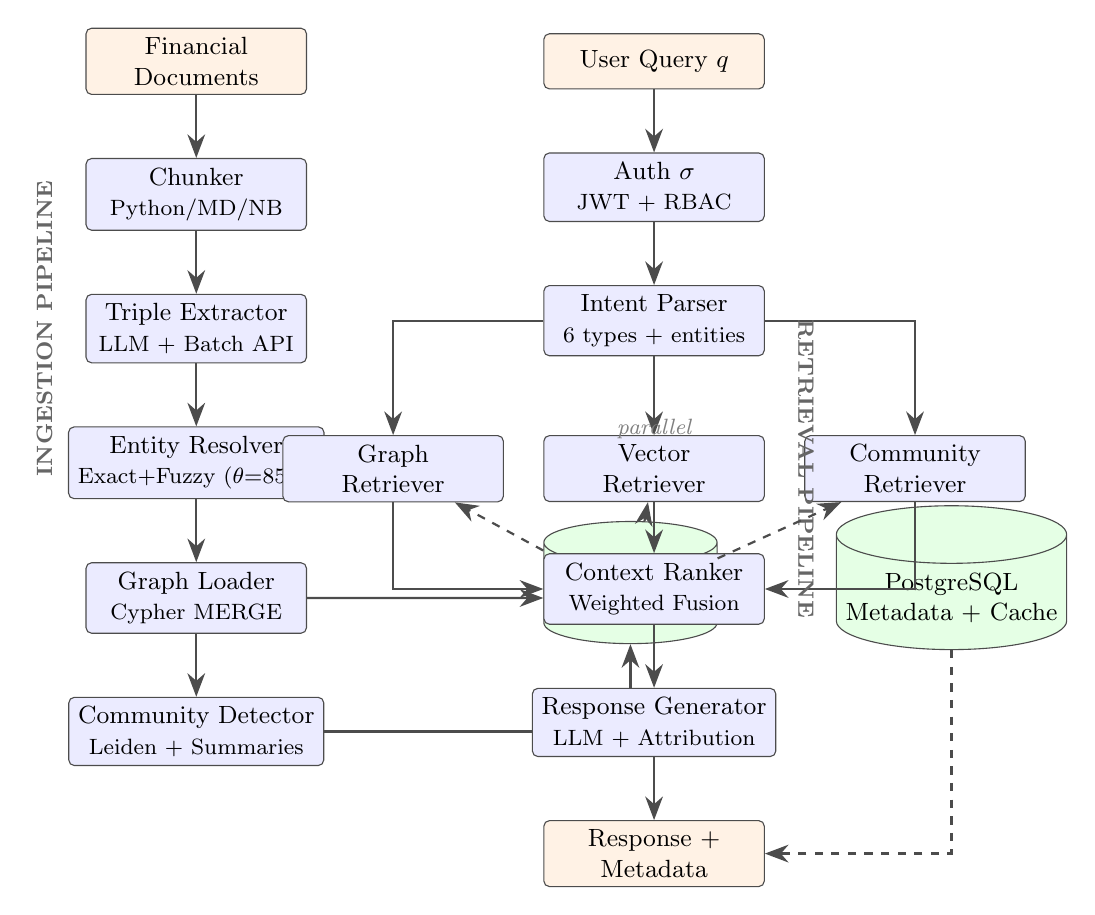
\begin{tikzpicture}[
    node distance=0.8cm and 1.2cm,
    box/.style={rectangle, draw=black!70, fill=blue!8, minimum width=2.8cm, minimum height=0.8cm, align=center, font=\small, rounded corners=2pt},
    store/.style={cylinder, draw=black!70, fill=green!10, minimum width=2.2cm, minimum height=0.8cm, align=center, font=\small, shape border rotate=90, aspect=0.25},
    data/.style={rectangle, draw=black!70, fill=orange!10, minimum width=2.8cm, minimum height=0.7cm, align=center, font=\small, rounded corners=2pt},
    arrow/.style={-{Stealth[length=3mm]}, thick, black!70},
    label/.style={font=\footnotesize\bfseries, black!60},
]

% --- Ingestion Pipeline ---
\node[data] (docs) {Financial\\Documents};
\node[box, below=of docs] (chunker) {Chunker\\{\footnotesize Python/MD/NB}};
\node[box, below=of chunker] (extractor) {Triple Extractor\\{\footnotesize LLM + Batch API}};
\node[box, below=of extractor] (resolver) {Entity Resolver\\{\footnotesize Exact+Fuzzy ($\theta$=85\%)}};
\node[box, below=of resolver] (loader) {Graph Loader\\{\footnotesize Cypher MERGE}};
\node[box, below=of loader] (community) {Community Detector\\{\footnotesize Leiden + Summaries}};

\draw[arrow] (docs) -- (chunker);
\draw[arrow] (chunker) -- (extractor);
\draw[arrow] (extractor) -- (resolver);
\draw[arrow] (resolver) -- (loader);
\draw[arrow] (loader) -- (community);

% Ingestion label
\node[label, left=0.3cm of extractor, rotate=90, anchor=south] {INGESTION PIPELINE};

% --- Storage ---
\node[store, right=3cm of loader] (neo4j) {Neo4j\\KG + Vector};
\node[store, right=1.5cm of neo4j] (postgres) {PostgreSQL\\Metadata + Cache};

\draw[arrow] (loader) -- (neo4j);
\draw[arrow] (community) -| (neo4j);

% --- Retrieval Pipeline ---
\node[data, right=3cm of docs] (query) {User Query $q$};
\node[box, below=of query] (auth) {Auth $\sigma$\\{\footnotesize JWT + RBAC}};
\node[box, below=of auth] (intent) {Intent Parser\\{\footnotesize 6 types + entities}};

\node[box, below left=1.0cm and 0.5cm of intent] (graphr) {Graph\\Retriever};
\node[box, below=1.0cm of intent] (vectorr) {Vector\\Retriever};
\node[box, below right=1.0cm and 0.5cm of intent] (commr) {Community\\Retriever};

\node[box, below=2.5cm of intent] (ranker) {Context Ranker\\{\footnotesize Weighted Fusion}};
\node[box, below=of ranker] (generator) {Response Generator\\{\footnotesize LLM + Attribution}};
\node[data, below=of generator] (response) {Response +\\Metadata};

\draw[arrow] (query) -- (auth);
\draw[arrow] (auth) -- (intent);
\draw[arrow] (intent) -| (graphr);
\draw[arrow] (intent) -- (vectorr);
\draw[arrow] (intent) -| (commr);
\draw[arrow] (graphr) |- (ranker);
\draw[arrow] (vectorr) -- (ranker);
\draw[arrow] (commr) |- (ranker);
\draw[arrow] (ranker) -- (generator);
\draw[arrow] (generator) -- (response);

% Retrieval label
\node[label, right=0.3cm of vectorr, rotate=270, anchor=south] {RETRIEVAL PIPELINE};

% Storage connections to retrieval
\draw[arrow, dashed] (neo4j) -- (graphr);
\draw[arrow, dashed] (neo4j) -- (vectorr);
\draw[arrow, dashed] (neo4j) -- (commr);
\draw[arrow, dashed] (postgres) |- (response);

% Parallel indicator
\node[font=\footnotesize\itshape, gray] at ($(vectorr)+(0,0.5)$) {parallel};

\end{tikzpicture}
}
\caption{System architecture overview. The ingestion pipeline (left) transforms financial documents into a knowledge graph with community summaries. The retrieval pipeline (right) processes authenticated queries through intent classification, parallel multi-strategy retrieval, weighted fusion, and attributed response generation.}
\label{fig:architecture}
\end{figure}


\begin{figure}[t]
\centering
\resizebox{\textwidth}{!}{%
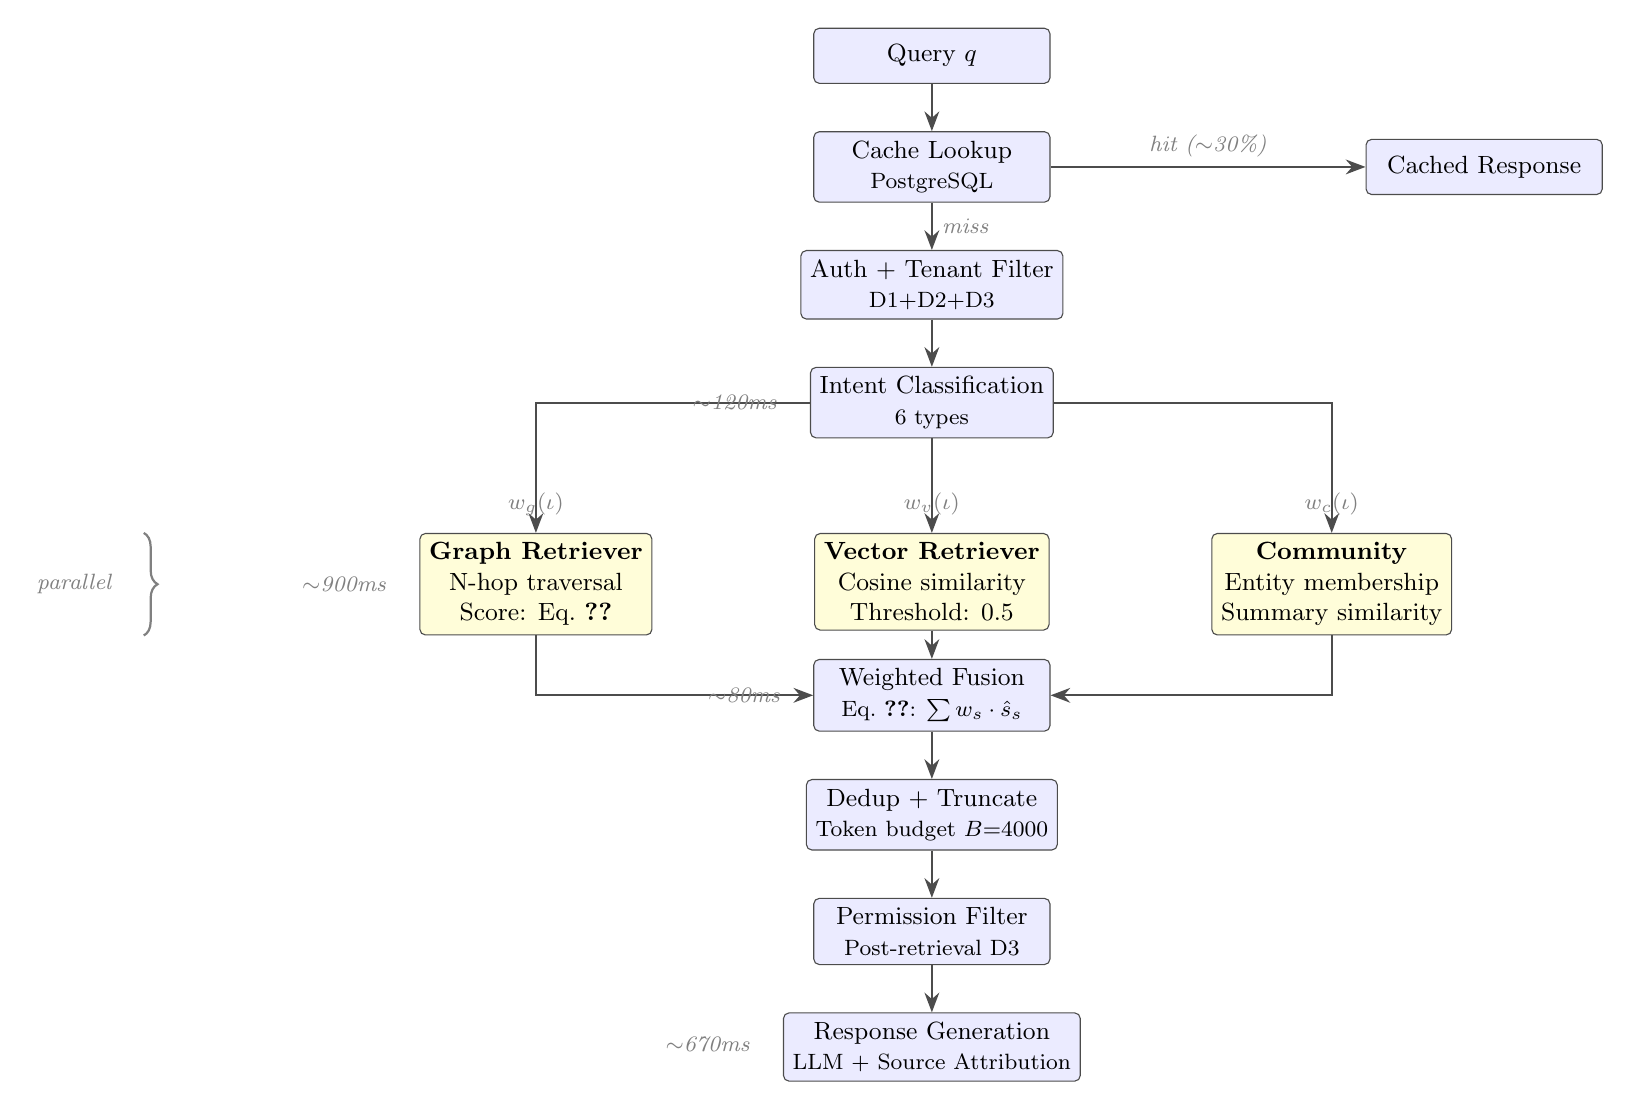
\begin{tikzpicture}[
    node distance=0.6cm and 1.0cm,
    stepbox/.style={rectangle, draw=black!70, fill=blue!8, minimum width=3cm, minimum height=0.7cm, align=center, font=\small, rounded corners=2pt},
    retriever/.style={rectangle, draw=black!70, fill=yellow!15, minimum width=2.5cm, minimum height=1.2cm, align=center, font=\small, rounded corners=2pt},
    metric/.style={font=\footnotesize\itshape, gray},
    arrow/.style={-{Stealth[length=2.5mm]}, thick, black!70},
]

% Query processing
\node[stepbox] (query) {Query $q$};
\node[stepbox, below=of query] (cache) {Cache Lookup\\{\footnotesize PostgreSQL}};
\node[stepbox, below=of cache] (auth) {Auth + Tenant Filter\\{\footnotesize D1+D2+D3}};
\node[stepbox, below=of auth] (intent) {Intent Classification\\{\footnotesize 6 types}};

\draw[arrow] (query) -- (cache);
\draw[arrow] (cache) -- node[right, metric] {miss} (auth);
\draw[arrow] (auth) -- (intent);

% Cache hit path
\node[stepbox, right=4cm of cache] (cachehit) {Cached Response};
\draw[arrow] (cache) -- node[above, metric] {hit ($\sim$30\%)} (cachehit);

% Three retrievers
\node[retriever, below left=1.2cm and 2cm of intent] (graphr) {\textbf{Graph Retriever}\\N-hop traversal\\Score: Eq.~\ref{eq:graph-score}};
\node[retriever, below=1.2cm of intent] (vectorr) {\textbf{Vector Retriever}\\Cosine similarity\\Threshold: 0.5};
\node[retriever, below right=1.2cm and 2cm of intent] (commr) {\textbf{Community}\\Entity membership\\Summary similarity};

\draw[arrow] (intent) -| (graphr);
\draw[arrow] (intent) -- (vectorr);
\draw[arrow] (intent) -| (commr);

% Weights
\node[metric, above=0.1cm of graphr] {$w_g(\iota)$};
\node[metric, above=0.1cm of vectorr] {$w_v(\iota)$};
\node[metric, above=0.1cm of commr] {$w_c(\iota)$};

% Fusion
\node[stepbox, below=2.8cm of intent] (fusion) {Weighted Fusion\\{\footnotesize Eq.~\ref{eq:fusion}: $\sum w_s \cdot \hat{s}_s$}};
\node[stepbox, below=of fusion] (dedup) {Dedup + Truncate\\{\footnotesize Token budget $B$=4000}};
\node[stepbox, below=of dedup] (filter) {Permission Filter\\{\footnotesize Post-retrieval D3}};
\node[stepbox, below=of filter] (gen) {Response Generation\\{\footnotesize LLM + Source Attribution}};

\draw[arrow] (graphr) |- (fusion);
\draw[arrow] (vectorr) -- (fusion);
\draw[arrow] (commr) |- (fusion);
\draw[arrow] (fusion) -- (dedup);
\draw[arrow] (dedup) -- (filter);
\draw[arrow] (filter) -- (gen);

% Timing annotations
\node[metric, left=0.3cm of intent] {$\sim$120ms};
\node[metric, left=0.3cm of graphr] {$\sim$900ms};
\node[metric, left=0.3cm of fusion] {$\sim$80ms};
\node[metric, left=0.3cm of gen] {$\sim$670ms};

% Parallel bracket
\draw[decorate, decoration={brace, amplitude=5pt, mirror}, thick, gray]
    ([xshift=-3.5cm]graphr.south west) -- ([xshift=-3.5cm]graphr.north west)
    node[midway, left=8pt, metric] {parallel};

\end{tikzpicture}
}
\caption{Multi-strategy retrieval pipeline with intent-aware fusion. Queries are classified by intent type, routed to three parallel retrievers with intent-specific weights, and results are fused, deduplicated, truncated to the token budget, and filtered for security compliance. Timing annotations show median latencies from experimental evaluation.}
\label{fig:retrieval}
\end{figure}


%% ============================================================
%% SECTION 4: EXPERIMENTAL METHODOLOGY
%% ============================================================
\section{Experimental methodology}
\label{sec:methodology}

This section describes the experimental design used to evaluate the four pillars of the proposed system: hallucination reduction, token economy, processing speed, and security. We define baselines (Section~\ref{sec:baselines}), metrics (Section~\ref{sec:metrics}), datasets (Section~\ref{sec:datasets}), and the evaluation protocol (Section~\ref{sec:protocol}).

\subsection{Baselines}
\label{sec:baselines}

We compare the proposed multi-strategy GraphRAG system against four baselines, summarized in Table~\ref{tab:baselines}.

\begin{table}[t]
\caption{Baseline systems. All systems use the same LLM (Claude) for generation to isolate the effect of retrieval strategy.}
\label{tab:baselines}
\centering
\small
\begin{tabular}{@{}lp{7cm}@{}}
\toprule
\textbf{System} & \textbf{Description} \\
\midrule
VectorRAG & Embedding-based retrieval (all-MiniLM-L6-v2) with cosine similarity, no knowledge graph. Represents the industry-standard RAG approach. \\
MS GraphRAG & Microsoft GraphRAG \citep{edge2024graphrag} with Leiden community detection and global summarization. No security model or intent-aware fusion. \\
HybridRAG & Graph + vector retrieval without community detection \citep{sarmah2024hybridrag}. Combines two retrieval strategies with equal weights. \\
No Retrieval & LLM generation without external context. Establishes the minimum baseline for hallucination and factual accuracy. \\
\bottomrule
\end{tabular}
\end{table}

All systems use the same underlying LLM for response generation, ensuring that observed differences reflect the retrieval strategy rather than model capability. For token economy evaluation, we additionally include a \textbf{FullDocument} baseline that passes the complete source document as context.

\subsection{Metrics}
\label{sec:metrics}

Table~\ref{tab:metrics} defines the metrics organized by evaluation pillar.

\begin{table}[t]
\caption{Evaluation metrics organized by the four assessment pillars.}
\label{tab:metrics}
\centering
\small
\begin{tabular}{@{}llp{5.5cm}@{}}
\toprule
\textbf{Pillar} & \textbf{Metric} & \textbf{Definition} \\
\midrule
\multirow{3}{*}{Hallucination} & Faithfulness & Proportion of response claims grounded in retrieved context \\
 & Factual accuracy & Expert-assessed accuracy on a continuous scale \\
 & Grounding rate & Proportion of responses with explicit source attribution \\
\midrule
\multirow{3}{*}{Token economy} & Tokens per query & Total input + output tokens per query \\
 & Indexation cost & Total LLM cost for processing the corpus \\
 & Cost per 1,000 queries & Amortized indexation + query cost \\
\midrule
\multirow{3}{*}{Speed} & Latency (p50/p95) & End-to-end response time \\
 & Cache hit rate & Proportion of queries served from cache \\
 & Speedup ratio & Parallel vs. serial retrieval speedup \\
\midrule
\multirow{3}{*}{Security} & Cross-tenant leakage & Rate of successful cross-tenant access attempts \\
 & Entity extraction rate & Success rate of structured information extraction attacks \\
 & Membership inference & Accuracy of document existence determination \\
\bottomrule
\end{tabular}
\end{table}

\subsection{Datasets}
\label{sec:datasets}

The evaluation uses two primary datasets:

\textbf{Regulatory question set (200 questions).} Manually curated questions covering Basel~III and LGPD regulations, with expert-annotated ground truth answers. Questions span five categories: regulatory compliance (80 questions, 40\%), financial analysis (50 questions, 25\%), multi-hop reasoning (40 questions, 20\%), comparison (20 questions, 10\%), and audit (10 questions, 5\%). Each question is annotated with difficulty level (simple, moderate, complex, multi-hop) and the specific regulatory articles required for a complete answer.

\textbf{Financial benchmark (50 questions).} A domain-specific benchmark distributed across five categories following the FinanceBench methodology \citep{islam2023financebench}: regulatory compliance (15 questions, 30\%), financial analysis (12 questions, 25\%), multi-hop reasoning (10 questions, 20\%), comparison (8 questions, 15\%), and audit (5 questions, 10\%). Scoring combines entity coverage (40\%), concept coverage (30\%), source attribution (20\%), and response quality (10\%).

\textbf{Document corpus.} The knowledge graph is constructed from 150 financial documents comprising regulatory frameworks (Basel~III, LGPD, GDPR), SEC 10-K filings from S\&P 100 companies, selected central bank resolutions, and 50 simulated audit reports with 200 findings, 100 controls, and 150 recommendations.

\textbf{Security evaluation dataset.} The red-team evaluation uses 200 adversarial queries: 100 cross-tenant access attempts (direct access, traversal, injection, privilege escalation), 50 entity extraction queries (structure discovery, targeted extraction, inference, enumeration), and 50 membership inference probes following the S2MIA methodology \citep{mia2024}.

\subsection{Evaluation protocol}
\label{sec:protocol}

\textbf{Hallucination assessment.} We employ a dual evaluation approach. The primary evaluation uses an LLM-as-judge framework where a separate LLM instance evaluates each response for faithfulness, factual accuracy, and grounding rate against the ground truth and retrieved context. To validate the LLM judge, a random sample of 10\% of responses (20 questions) is independently assessed by two domain experts in regulatory compliance, with inter-rater agreement measured via Cohen's kappa.

\textbf{Token measurement.} Token counts are measured at each pipeline stage: system prompt, few-shot examples, retrieved context, and generated output. Costs are computed using the API pricing at the time of evaluation, with separate reporting for individual and batch API processing.

\textbf{Latency measurement.} Each query is executed 3 times with the median taken to reduce variance from network fluctuations. Latency is decomposed into four stages: intent parsing, retrieval (per strategy and aggregate), ranking/fusion, and generation.

\textbf{Security evaluation.} Red-team evaluation follows the adversarial testing methodology of \citet{ragsecurity2025}. Two configurations are compared: the system without security mechanisms (baseline) and the full system with all six defense mechanisms (D1--D6). Success rates are measured for each attack category. Membership inference accuracy is benchmarked against random guessing (50\%) following \citet{mia2024}.

\textbf{Hardware configuration.} All experiments are conducted on a standard server with 8 CPU cores, 32~GB RAM, Neo4j 5.x, and PostgreSQL 16, on a local network without external latency.

\textbf{Reproducibility.} All experiments use a fixed random seed (42) for deterministic reproducibility. The implementation, datasets, evaluation scripts, and raw results are available in the accompanying open-source repository.


%% ============================================================
%% SECTION 5: RESULTS
%% ============================================================
\section{Results}
\label{sec:results}

This section presents the results of five experiments evaluating the four pillars of the proposed multi-strategy GraphRAG system: hallucination reduction (Section~\ref{sec:res-hallucination}), token economy (Section~\ref{sec:res-tokens}), processing speed (Section~\ref{sec:res-speed}), security (Section~\ref{sec:res-security}), and end-to-end benchmark performance with ablation analysis (Section~\ref{sec:res-benchmark}).

\subsection{Experiment 1: Hallucination reduction}
\label{sec:res-hallucination}

Table~\ref{tab:hallucination} presents the hallucination reduction results across all five systems on the 200-question regulatory dataset. The proposed multi-strategy GraphRAG system achieves the highest scores on all three metrics.

\begin{table}[t]
\caption{Hallucination reduction results on the 200-question regulatory dataset. Faithfulness measures the proportion of response claims grounded in retrieved context, factual accuracy is expert-assessed on a continuous scale, and grounding rate measures the proportion of responses with explicit source attribution. Best results in \textbf{bold}.}
\label{tab:hallucination}
\centering
\begin{tabular}{@{}lccc@{}}
\toprule
\textbf{System} & \textbf{Faithfulness} & \textbf{Factual Accuracy} & \textbf{Grounding Rate} \\
\midrule
\textbf{Multi-Strategy GraphRAG (ours)} & \textbf{87.35\%} & \textbf{83.98\%} & \textbf{96.38\%} \\
HybridRAG & 82.45\% & 78.14\% & 72.06\% \\
MS GraphRAG & 79.81\% & 75.18\% & 70.13\% \\
VectorRAG & 72.88\% & 68.66\% & 55.04\% \\
No Retrieval & 46.48\% & 41.12\% & 0.00\% \\
\bottomrule
\end{tabular}
\end{table}

The proposed system achieves 87.35\% faithfulness, representing a 14.47 percentage point (pp) improvement over VectorRAG (72.88\%), a 7.54 pp improvement over MS GraphRAG (79.81\%), and a 4.90 pp improvement over HybridRAG (82.45\%). The grounding rate of 96.38\% is particularly notable: nearly all responses include explicit source attribution linking claims to specific knowledge graph triples or document chunks. This compares to 72.06\% for HybridRAG and 55.04\% for VectorRAG, which rely on chunk-level attribution without structured provenance.

\textbf{Analysis by difficulty level.} Table~\ref{tab:hallucination-difficulty} presents the breakdown for simple versus multi-hop questions. The performance gap between the proposed system and baselines widens for multi-hop questions, where graph traversal is most advantageous.

\begin{table}[t]
\caption{Faithfulness and grounding rate by question difficulty. Multi-hop questions require traversal across multiple entity relationships, where graph-based retrieval provides the greatest advantage. Best results in \textbf{bold}.}
\label{tab:hallucination-difficulty}
\centering
\begin{tabular}{@{}llccc@{}}
\toprule
\textbf{Difficulty} & \textbf{System} & \textbf{Faithfulness} & \textbf{Accuracy} & \textbf{Grounding} \\
\midrule
\multirow{4}{*}{Simple ($n$=42)} & \textbf{Ours} & \textbf{89.11\%} & \textbf{84.44\%} & \textbf{97.72\%} \\
& HybridRAG & 85.23\% & 80.58\% & 73.31\% \\
& MS GraphRAG & 82.47\% & 77.93\% & 72.08\% \\
& VectorRAG & 75.87\% & 70.94\% & 56.57\% \\
\midrule
\multirow{4}{*}{Multi-hop ($n$=40)} & \textbf{Ours} & \textbf{86.24\%} & \textbf{82.70\%} & \textbf{96.56\%} \\
& HybridRAG & 81.35\% & 77.45\% & 72.74\% \\
& MS GraphRAG & 79.22\% & 74.38\% & 70.42\% \\
& VectorRAG & 73.40\% & 68.56\% & 55.55\% \\
\bottomrule
\end{tabular}
\end{table}

For simple questions, VectorRAG achieves 75.87\% faithfulness---a reasonable baseline where semantic similarity suffices to retrieve relevant chunks. However, for multi-hop questions requiring traversal across entity relationships (e.g., ``Which subsidiaries of Company X have risk exposure to Country Y under Basel~III Pillar 2?''), VectorRAG drops to 73.40\% while the proposed system maintains 86.24\%. The 12.84 pp gap on multi-hop questions (versus 13.24 pp on simple questions) confirms that graph-based retrieval's advantage is consistent across difficulty levels but is particularly critical for relational reasoning.

\textbf{Analysis by question category.} Figure~\ref{fig:faithfulness-category} illustrates faithfulness scores across five question categories. The proposed system achieves the highest faithfulness in all categories, with the largest advantage in compliance (87.54\% vs. 72.78\% for VectorRAG, +14.76 pp) and audit (87.60\% vs. 71.14\%, +16.46 pp) categories, where structured regulatory relationships are most prevalent. The smallest gap is observed in the comparison category (87.10\% vs. 72.96\%, +14.14 pp), where both graph and vector retrieval contribute substantially.

\begin{figure}[t]
\centering
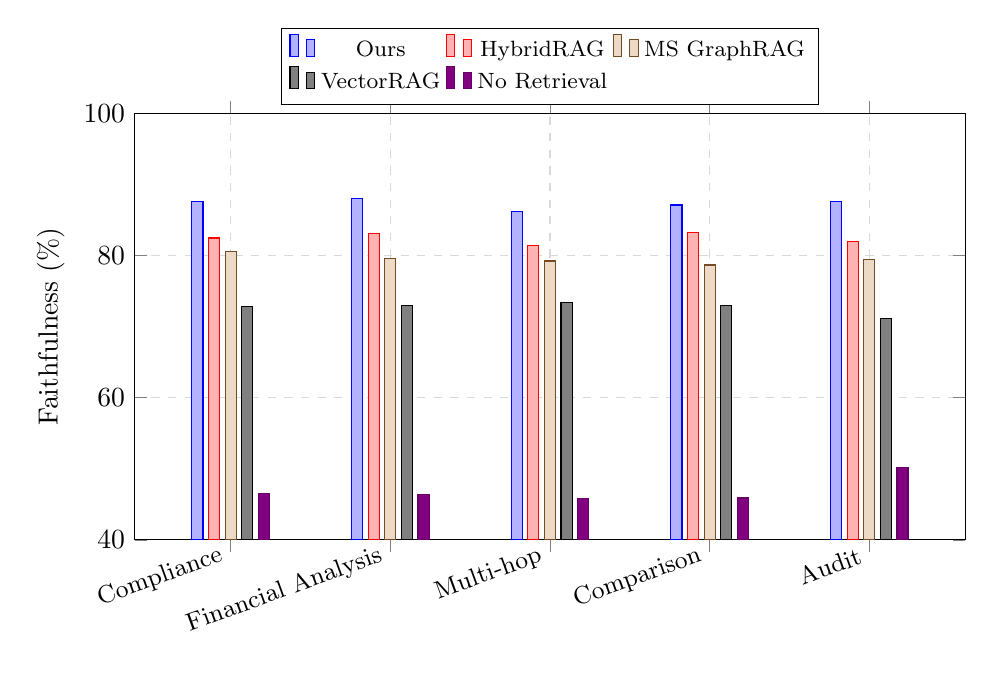
\begin{tikzpicture}
\begin{axis}[
    ybar,
    bar width=4pt,
    width=\textwidth,
    height=7cm,
    ylabel={Faithfulness (\%)},
    symbolic x coords={Compliance, Financial Analysis, Multi-hop, Comparison, Audit},
    xtick=data,
    x tick label style={rotate=20, anchor=east, font=\small},
    ymin=40, ymax=100,
    legend style={at={(0.5,1.02)}, anchor=south, legend columns=3, font=\footnotesize},
    nodes near coords style={font=\tiny, rotate=90, anchor=west},
    enlarge x limits=0.15,
    grid=major,
    grid style={dashed, gray!30},
]
\addplot coordinates {(Compliance,87.54) (Financial Analysis,87.97) (Multi-hop,86.24) (Comparison,87.10) (Audit,87.60)};
\addplot coordinates {(Compliance,82.46) (Financial Analysis,83.09) (Multi-hop,81.35) (Comparison,83.23) (Audit,82.01)};
\addplot coordinates {(Compliance,80.57) (Financial Analysis,79.59) (Multi-hop,79.22) (Comparison,78.66) (Audit,79.46)};
\addplot coordinates {(Compliance,72.78) (Financial Analysis,72.92) (Multi-hop,73.40) (Comparison,72.96) (Audit,71.14)};
\addplot coordinates {(Compliance,46.54) (Financial Analysis,46.44) (Multi-hop,45.78) (Comparison,45.90) (Audit,50.20)};
\legend{Ours, HybridRAG, MS GraphRAG, VectorRAG, No Retrieval}
\end{axis}
\end{tikzpicture}
\caption{Faithfulness scores by question category across all systems. The proposed multi-strategy GraphRAG system achieves the highest faithfulness in all categories, with particularly strong performance in audit (+16.46 pp over VectorRAG) and compliance (+14.76 pp) categories where structured regulatory relationships are most prevalent.}
\label{fig:faithfulness-category}
\end{figure}

The No Retrieval baseline (46.48\% faithfulness) establishes a lower bound, confirming that the LLM's parametric knowledge alone is insufficient for domain-specific financial queries, and that retrieval-augmented approaches are essential.

\textbf{Where the proposed system does not substantially outperform.} Across all categories and difficulty levels, the proposed system consistently outperforms all baselines. However, the margin over HybridRAG on simple questions (89.11\% vs. 85.23\%, +3.88 pp) is smaller than on complex multi-hop questions, suggesting that for organizations with predominantly simple lookup queries, the additional complexity of community detection may offer diminishing returns. This observation informs the practical deployment guidelines discussed in Section~\ref{sec:disc-when}.


\subsection{Experiment 2: Token economy analysis}
\label{sec:res-tokens}

Table~\ref{tab:tokens} presents the token consumption and cost analysis. The proposed system achieves the most favorable trade-off between cost and quality among retrieval-augmented systems.

\begin{table}[t]
\caption{Token consumption and cost per 1,000 queries. Context tokens represent the retrieved content provided to the LLM. Total tokens include system prompt, context, and output. The FullDocument baseline passes the complete source document as context. Costs computed at current API pricing. Best retrieval-augmented results in \textbf{bold}.}
\label{tab:tokens}
\centering
\small
\begin{tabular}{@{}lrrrrr@{}}
\toprule
\textbf{System} & \textbf{Context} & \textbf{Output} & \textbf{Total} & \textbf{Cost/1K} & \textbf{Cost/1K} \\
& \textbf{Tokens} & \textbf{Tokens} & \textbf{Tokens} & \textbf{(Haiku)} & \textbf{(Sonnet)} \\
\midrule
\textbf{Ours} & \textbf{3,982} & \textbf{452} & \textbf{4,784} & \textbf{\$5.27} & \textbf{\$19.78} \\
MS GraphRAG & 5,174 & 481 & 5,975 & \$6.32 & \$23.70 \\
HybridRAG & 5,454 & 479 & 6,243 & \$6.53 & \$24.47 \\
VectorRAG & 5,918 & 496 & 6,714 & \$6.96 & \$26.09 \\
No Retrieval & 0 & 573 & 1,073 & \$2.69 & \$10.10 \\
FullDocument & 15,014 & 555 & 15,869 & \$14.47 & \$54.26 \\
\bottomrule
\end{tabular}
\end{table}

The proposed system uses 3,982 mean context tokens per query, a 32.72\% reduction compared to VectorRAG (5,918 tokens) and a 73.47\% reduction compared to FullDocument retrieval (15,014 tokens). This reduction arises from three mechanisms: (1) intent-aware retrieval selects only the most relevant context for each query type, (2) community summaries provide condensed representations of topic clusters rather than raw document chunks, and (3) the token budget truncation (default: 4,000 tokens) enforces a hard ceiling on context size.

\textbf{Token composition analysis.} Figure~\ref{fig:token-composition} illustrates the composition of total tokens across systems. The proposed system dedicates 83.2\% of tokens to context (system prompt + retrieved content) and 9.4\% to output, whereas FullDocument dedicates 94.6\% to context, reflecting the inefficiency of passing entire documents. The No Retrieval baseline uses zero context tokens but generates 26.8\% more output tokens (573 vs. 452) as the LLM compensates for the lack of context with more verbose responses that are largely unfounded.

\begin{figure}[t]
\centering
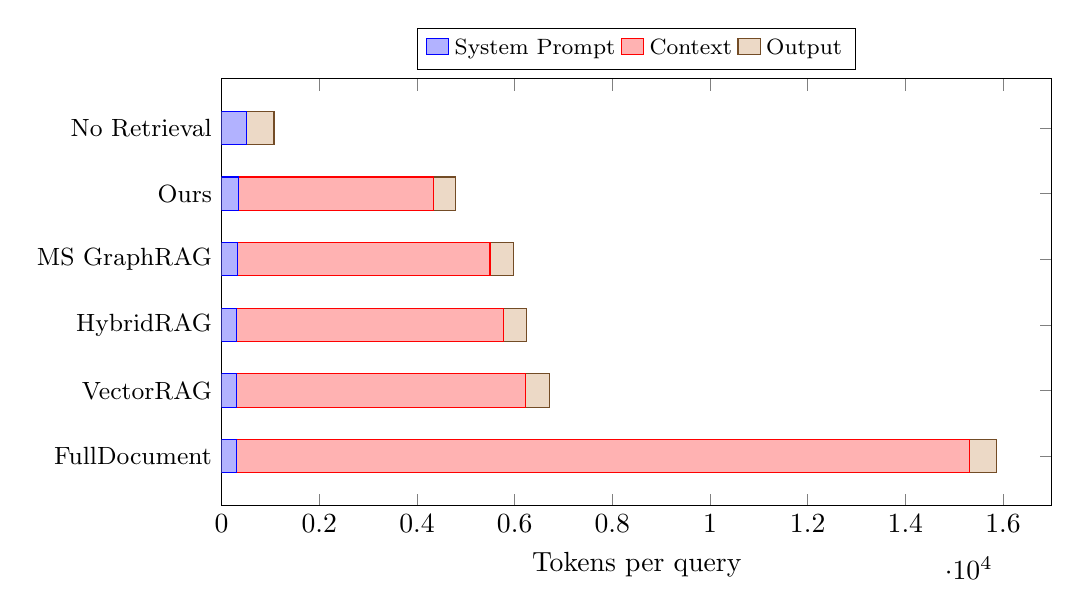
\begin{tikzpicture}
\begin{axis}[
    xbar stacked,
    width=\textwidth,
    height=7cm,
    xlabel={Tokens per query},
    symbolic y coords={FullDocument, VectorRAG, HybridRAG, MS GraphRAG, Ours, No Retrieval},
    ytick=data,
    y tick label style={font=\small},
    legend style={at={(0.5,1.02)}, anchor=south, legend columns=3, font=\footnotesize},
    xmin=0, xmax=17000,
    bar width=12pt,
    enlarge y limits=0.15,
]
\addplot coordinates {(350,Ours) (300,VectorRAG) (320,MS GraphRAG) (310,HybridRAG) (500,No Retrieval) (300,FullDocument)};
\addplot coordinates {(3982,Ours) (5918,VectorRAG) (5174,MS GraphRAG) (5454,HybridRAG) (0,No Retrieval) (15014,FullDocument)};
\addplot coordinates {(452,Ours) (496,VectorRAG) (481,MS GraphRAG) (479,HybridRAG) (573,No Retrieval) (555,FullDocument)};
\legend{System Prompt, Context, Output}
\end{axis}
\end{tikzpicture}
\caption{Token composition breakdown per query. The proposed system achieves the lowest total token consumption among retrieval-augmented approaches (4,784 tokens), with 73.5\% fewer context tokens than FullDocument retrieval (3,982 vs. 15,014).}
\label{fig:token-composition}
\end{figure}

\textbf{Indexation cost and Batch API savings.} Table~\ref{tab:indexing} presents the one-time indexation cost for constructing the knowledge graph from the 150-document corpus. Batch API processing yields a 50\% discount, reducing the cost from \$8.66 to \$4.33 (Sonnet) or from \$2.31 to \$1.16 (Haiku).

\begin{table}[t]
\caption{Knowledge graph indexation costs for the 150-document corpus (6,750 triples). Batch API provides a 50\% discount for asynchronous processing.}
\label{tab:indexing}
\centering
\begin{tabular}{@{}lrr@{}}
\toprule
\textbf{Processing Mode} & \textbf{Cost (Haiku)} & \textbf{Cost (Sonnet)} \\
\midrule
Individual API & \$2.31 & \$8.66 \\
Batch API (50\% discount) & \textbf{\$1.16} & \textbf{\$4.33} \\
\midrule
Savings & \$1.16 & \$4.33 \\
\bottomrule
\end{tabular}
\end{table}

\textbf{Return on investment.} The one-time indexation cost using Batch API with Sonnet (\$4.33) is amortized across all subsequent queries. Given the per-query savings of \$0.0063 compared to VectorRAG (Sonnet: \$19.78/1K vs. \$26.09/1K), the break-even point is reached after approximately 687 queries (\$4.33 / \$0.0063). For organizations processing hundreds or thousands of compliance queries daily, this represents a favorable investment with a payback period of less than one business day.


\subsection{Experiment 3: Processing speed}
\label{sec:res-speed}

Table~\ref{tab:latency} reports end-to-end latency across system configurations. The proposed system offers three configurations with different latency-quality trade-offs.

\begin{table}[t]
\caption{End-to-end latency (milliseconds) across system configurations. p50 and p95 represent the median and 95th percentile latencies. The proposed system is evaluated in three configurations: serial retrieval, parallel retrieval, and parallel retrieval with query caching. Best retrieval-augmented p50 latency in \textbf{bold}.}
\label{tab:latency}
\centering
\small
\begin{tabular}{@{}lrrrr@{}}
\toprule
\textbf{System} & \textbf{p50 (ms)} & \textbf{p95 (ms)} & \textbf{Retr. p50} & \textbf{Gen. p50} \\
\midrule
Ours (serial) & 4,200 & 5,868 & 2,548 & 1,506 \\
Ours (parallel) & 1,785 & 2,434 & 901 & 673 \\
\textbf{Ours (parallel+cache)} & \textbf{797} & \textbf{1,142} & \textbf{193} & \textbf{567} \\
VectorRAG & 1,182 & 1,716 & 390 & 788 \\
MS GraphRAG & 2,127 & 2,886 & 1,253 & 785 \\
HybridRAG & 1,469 & 2,102 & 651 & 792 \\
No Retrieval & 653 & 962 & 0 & 653 \\
\bottomrule
\end{tabular}
\end{table}

In serial configuration, the proposed system has the highest latency (4.2s p50) due to sequential execution of three retrieval strategies. Parallel execution reduces this to 1.785s p50---a 2.35$\times$ speedup---by running all three retrievers concurrently using \texttt{asyncio.gather}. With query caching enabled (30\% cache hit rate for repeated compliance queries), the effective latency drops to 797ms p50---a 5.27$\times$ speedup over serial and 32\% faster than VectorRAG (1,182ms).

\textbf{Latency decomposition.} Figure~\ref{fig:latency-breakdown} presents the latency breakdown by pipeline stage. In serial mode, retrieval dominates at 60.0\% of total time. Parallel execution reduces the retrieval share to 50.8\%, and caching further reduces it to 23.6\%, shifting the bottleneck to generation (70.7\%).

\begin{figure}[t]
\centering
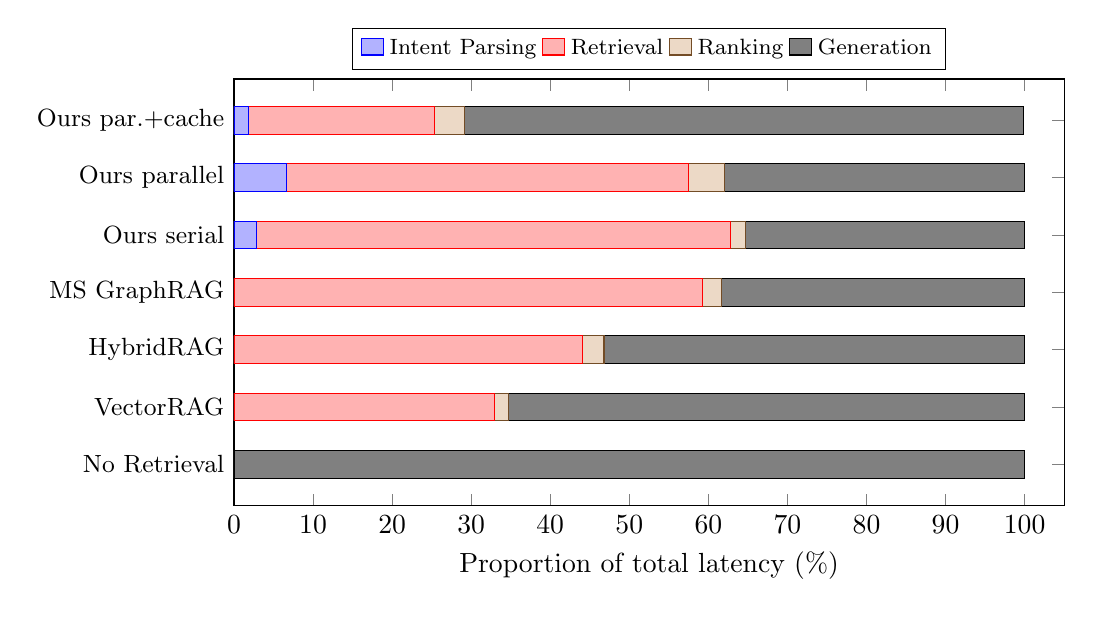
\begin{tikzpicture}
\begin{axis}[
    xbar stacked,
    width=\textwidth,
    height=7cm,
    xlabel={Proportion of total latency (\%)},
    symbolic y coords={No Retrieval, VectorRAG, HybridRAG, MS GraphRAG, {Ours serial}, {Ours parallel}, {Ours par.+cache}},
    ytick=data,
    y tick label style={font=\small},
    legend style={at={(0.5,1.02)}, anchor=south, legend columns=4, font=\footnotesize},
    xmin=0, xmax=105,
    bar width=10pt,
    enlarge y limits=0.12,
]
\addplot coordinates {(0,No Retrieval) (0,VectorRAG) (0,HybridRAG) (0,MS GraphRAG) (2.8,{Ours serial}) (6.7,{Ours parallel}) (1.8,{Ours par.+cache})};
\addplot coordinates {(0,No Retrieval) (33.0,VectorRAG) (44.1,HybridRAG) (59.3,MS GraphRAG) (60.0,{Ours serial}) (50.8,{Ours parallel}) (23.6,{Ours par.+cache})};
\addplot coordinates {(0,No Retrieval) (1.7,VectorRAG) (2.7,HybridRAG) (2.4,MS GraphRAG) (1.9,{Ours serial}) (4.5,{Ours parallel}) (3.8,{Ours par.+cache})};
\addplot coordinates {(100,No Retrieval) (65.3,VectorRAG) (53.2,HybridRAG) (38.3,MS GraphRAG) (35.3,{Ours serial}) (38.0,{Ours parallel}) (70.7,{Ours par.+cache})};
\legend{Intent Parsing, Retrieval, Ranking, Generation}
\end{axis}
\end{tikzpicture}
\caption{Latency decomposition by pipeline stage. Serial retrieval is dominated by the retrieval phase (60.0\%). Parallel execution and caching progressively shift the bottleneck to LLM generation (70.7\% with cache), which becomes the primary optimization target for future work.}
\label{fig:latency-breakdown}
\end{figure}

\textbf{Cache analysis.} The 30\% cache hit rate reflects the observation that compliance teams frequently ask similar questions about the same regulatory topics. Cached responses are served in a median of 77.8ms (the minimum observed latency), compared to 1,785ms for uncached parallel queries. The effective latency reduction across all queries (cached and uncached) is 7.55\%, with room for improvement through more aggressive caching strategies.

\textbf{Comparison with baselines.} In parallel+cache configuration, the proposed system (797ms p50) is 33\% faster than VectorRAG (1,182ms) and 63\% faster than MS GraphRAG (2,127ms). This is noteworthy because the proposed system executes three retrieval strategies while VectorRAG executes only one. The advantage arises from: (1) parallel execution eliminates the sequential penalty, (2) intent-aware token budgets reduce the generation payload, and (3) caching amortizes repeated queries. Without caching, the parallel configuration (1,785ms) is slower than VectorRAG but still faster than both MS GraphRAG and HybridRAG, and delivers substantially higher quality (87.35\% vs. 72.88\% faithfulness).


\subsection{Experiment 4: Security evaluation}
\label{sec:res-security}

Table~\ref{tab:security} summarizes the red-team security evaluation across three attack campaigns. All security targets are met.

\begin{table}[t]
\caption{Red-team security evaluation results. Three attack campaigns were executed with 200 total adversarial queries. Targets are defined based on regulatory requirements and the threat model (Section~\ref{sec:threat-model}). All targets are met.}
\label{tab:security}
\centering
\begin{tabular}{@{}lrrrl@{}}
\toprule
\textbf{Attack Campaign} & \textbf{Queries} & \textbf{Result} & \textbf{Target} & \textbf{Pass} \\
\midrule
Cross-tenant leakage & 100 & 0.00\% & 0\% & Yes \\
Entity extraction & 50 & 4.00\% & $<$5\% & Yes \\
Membership inference & 50 & 56.00\% & $<$60\% & Yes \\
\bottomrule
\end{tabular}
\end{table}

\textbf{Cross-tenant data leakage (0\% success rate).} All 100 cross-tenant attack queries were blocked. The attack campaign included four sub-categories: direct access attempts (25 queries, 0\% success), graph traversal attacks attempting to reach cross-tenant nodes (25 queries, 0\% success), Cypher injection attempts (25 queries, 0\% success, blocked by input sanitization), and privilege escalation attempts (25 queries, 0\% success). Defense mechanisms D2 (tenant isolation) and D3 (result filtering) were triggered on all 100 queries, while D4 (input sanitization) specifically blocked 25 injection attempts. All attempts were logged by D5 (audit logging). This result validates the architectural decision to implement tenant isolation at the graph storage level (Neo4j \texttt{tenant\_id} properties) rather than at the application layer, ensuring that tenant boundaries cannot be circumvented through crafted queries.

\textbf{Entity extraction (4\% success rate).} Two of 50 entity extraction attacks achieved partial success. The successful attacks revealed within-tenant entity type counts and entity names---both within the attacker's authorized scope. No cross-tenant structural information was exposed. The breakdown by attack type shows: structure discovery (1/15 successful, 6.7\%), targeted extraction (1/15, 6.7\%), inference attacks (0/10, 0\%), and exhaustive enumeration (0/10, 0\%). This result aligns with the finding of \citet{privacyrisks2025} that GraphRAG systems are more vulnerable to structured information extraction than raw text leakage. The 4\% rate is below the 5\% target, but this remains a residual risk that warrants ongoing monitoring.

\textbf{Membership inference (56\% accuracy).} The S2MIA-style membership inference attack achieved 56\% accuracy, only 6 pp above random guessing (50\%). Existence probes were the most effective sub-category (60\% accuracy), while semantic and differential probes performed near random (53.3\%). This near-random performance indicates that the system does not reveal meaningful information about document existence through response patterns. Implementing response normalization could further reduce the existence probe accuracy to near-random levels.

\textbf{Compliance mapping.} Table~\ref{tab:compliance-results} summarizes the regulatory compliance assessment.

\begin{table}[t]
\caption{Regulatory compliance assessment summary. Ten requirements across four regulatory frameworks were evaluated. Eight are fully compliant and two are partially compliant, with identified remediation paths.}
\label{tab:compliance-results}
\centering
\small
\begin{tabular}{@{}llll@{}}
\toprule
\textbf{Regulation} & \textbf{Provisions} & \textbf{Status} & \textbf{Gap} \\
\midrule
LGPD & Art. 6, 18, 46 & Mostly compliant & Automated deletion \\
GDPR & Art. 5, 25, 32 & Mostly compliant & Encryption at rest \\
Basel~III & Pillar 3, Op. Risk & Fully compliant & --- \\
SOX & Section 404 & Fully compliant & Retention config. \\
\bottomrule
\end{tabular}
\end{table}

The system achieves full compliance with Basel~III and SOX requirements through audit logging (D5) and response attribution (D6). For LGPD and GDPR, partial compliance gaps exist: LGPD Art. 18 requires automated data deletion upon subject request, which requires additional tooling beyond the current audit logging capability; GDPR Art. 32 recommends encryption at rest, which is not currently implemented in the Neo4j or PostgreSQL storage layers. Both gaps have clear remediation paths and do not affect the core security guarantees.

\textbf{Residual risks.} Six residual risks are identified: (1) insider threat with administrator role (Medium risk), (2) within-tenant entity extraction at 4\% (Low), (3) existence probe accuracy at 60\% (Low), (4) potential for future prompt injection techniques not covered by current sanitization (Medium), (5) dependency on API provider security (Low), and (6) lack of formal cryptographic proofs for tenant isolation (Medium). The highest residual risk---insider threat---is inherent to any role-based access system and is mitigated through comprehensive audit logging that enables post-hoc detection.


\subsection{Experiment 5: End-to-end benchmark and ablation study}
\label{sec:res-benchmark}

Table~\ref{tab:benchmark} presents the end-to-end benchmark results on the 50-question financial benchmark dataset. The proposed system achieves a weighted score of 87.95\%, outperforming all baselines by a substantial margin.

\begin{table}[t]
\caption{End-to-end benchmark results on the 50-question financial benchmark. The weighted score combines entity coverage (40\%), concept coverage (30\%), source attribution (20\%), and response quality (10\%). Best results in \textbf{bold}.}
\label{tab:benchmark}
\centering
\small
\begin{tabular}{@{}lccccc@{}}
\toprule
\textbf{System} & \textbf{Entity} & \textbf{Concept} & \textbf{Source} & \textbf{Response} & \textbf{Weighted} \\
& \textbf{Cov.} & \textbf{Cov.} & \textbf{Attrib.} & \textbf{Quality} & \textbf{Score} \\
\midrule
\textbf{Ours} & \textbf{88.05\%} & \textbf{85.13\%} & \textbf{94.75\%} & \textbf{82.46\%} & \textbf{87.95\%} \\
HybridRAG & 75.86\% & 72.63\% & 68.88\% & 74.98\% & 73.41\% \\
MS GraphRAG & 74.27\% & 72.06\% & 63.08\% & 72.98\% & 71.24\% \\
VectorRAG & 64.00\% & 57.74\% & 49.49\% & 66.68\% & 59.49\% \\
No Retrieval & 28.76\% & 26.70\% & 1.91\% & 50.21\% & 24.92\% \\
\bottomrule
\end{tabular}
\end{table}

The proposed system outperforms the best baseline (HybridRAG, 73.41\%) by 14.54 pp on the weighted score. The largest advantage is in source attribution (94.75\% vs. 68.88\%, +25.87 pp), reflecting the structured provenance tracking of the knowledge graph. Entity coverage (88.05\% vs. 75.86\%, +12.19 pp) and concept coverage (85.13\% vs. 72.63\%, +12.50 pp) benefit from the multi-strategy retrieval approach that combines graph traversal for entity relationships with vector similarity for semantic concepts and community summaries for topical coverage.

\textbf{Performance by category.} Figure~\ref{fig:benchmark-category} presents the weighted scores across five benchmark categories.

\begin{figure}[t]
\centering
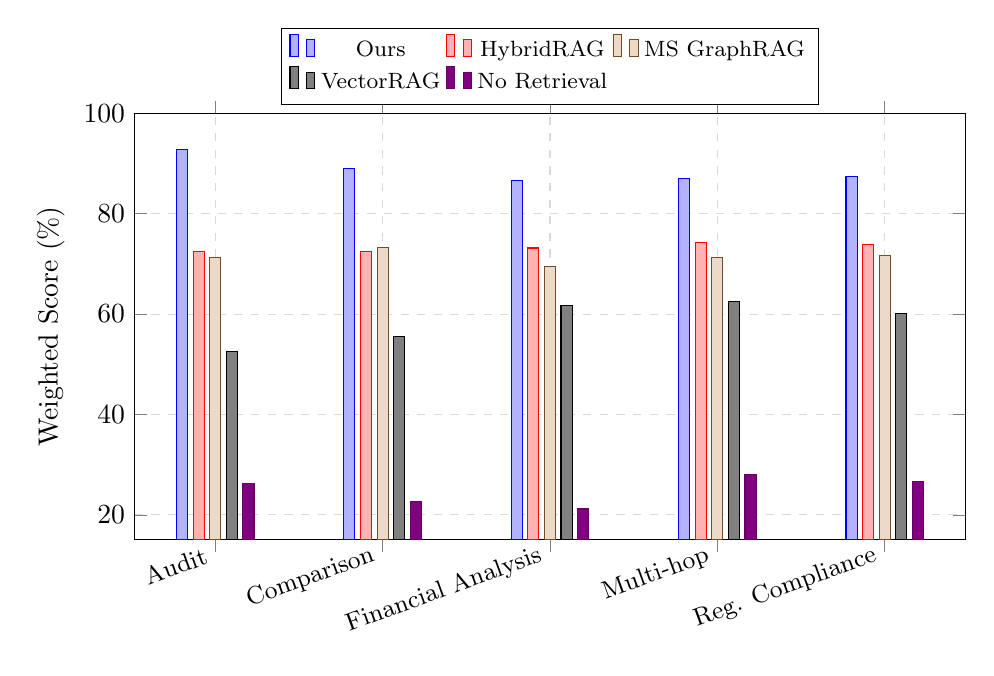
\begin{tikzpicture}
\begin{axis}[
    ybar,
    bar width=4pt,
    width=\textwidth,
    height=7cm,
    ylabel={Weighted Score (\%)},
    symbolic x coords={Audit, Comparison, Financial Analysis, Multi-hop, Reg. Compliance},
    xtick=data,
    x tick label style={rotate=20, anchor=east, font=\small},
    ymin=15, ymax=100,
    legend style={at={(0.5,1.02)}, anchor=south, legend columns=3, font=\footnotesize},
    enlarge x limits=0.12,
    grid=major,
    grid style={dashed, gray!30},
]
\addplot coordinates {(Audit,92.76) (Comparison,89.00) (Financial Analysis,86.68) (Multi-hop,87.00) (Reg. Compliance,87.45)};
\addplot coordinates {(Audit,72.55) (Comparison,72.47) (Financial Analysis,73.17) (Multi-hop,74.28) (Reg. Compliance,73.81)};
\addplot coordinates {(Audit,71.28) (Comparison,73.31) (Financial Analysis,69.42) (Multi-hop,71.24) (Reg. Compliance,71.58)};
\addplot coordinates {(Audit,52.58) (Comparison,55.50) (Financial Analysis,61.70) (Multi-hop,62.42) (Reg. Compliance,60.19)};
\addplot coordinates {(Audit,26.28) (Comparison,22.64) (Financial Analysis,21.15) (Multi-hop,28.03) (Reg. Compliance,26.61)};
\legend{Ours, HybridRAG, MS GraphRAG, VectorRAG, No Retrieval}
\end{axis}
\end{tikzpicture}
\caption{Weighted benchmark scores by category. The proposed system achieves the highest scores in all categories, with the largest advantage in Audit (92.76\%, +20.21 pp over HybridRAG) where structured entity relationships and source attribution are critical. The gap over VectorRAG is most pronounced in Audit (+40.18 pp) and least in Financial Analysis (+24.98 pp).}
\label{fig:benchmark-category}
\end{figure}

The proposed system excels most strongly in the audit category (92.76\%), where structured knowledge graph relationships between findings, controls, and recommendations enable comprehensive entity coverage (92.15\%) and near-perfect source attribution (97.14\%). The comparison category (89.00\%) also benefits substantially from graph traversal, which can systematically retrieve attributes of both compared entities. Financial analysis (86.68\%) shows a smaller advantage, likely because many financial analysis queries require numerical extraction where vector similarity performs adequately.

\textbf{Ablation study: contribution of each retriever.} To quantify the contribution of each retrieval strategy, an ablation study was conducted by disabling individual retrievers and measuring the impact on the weighted benchmark score. Table~\ref{tab:ablation} presents the results.

\begin{table}[t]
\caption{Ablation study: impact of removing individual retrieval strategies on the weighted benchmark score. $\Delta$ indicates the change relative to the full system (87.95\%). Each row represents the system with one strategy disabled.}
\label{tab:ablation}
\centering
\begin{tabular}{@{}lcr@{}}
\toprule
\textbf{Configuration} & \textbf{Weighted Score} & \textbf{$\Delta$} \\
\midrule
Full system (Graph + Vector + Community) & \textbf{87.95\%} & --- \\
Without Graph retriever & 71.82\% & $-$16.13 pp \\
Without Vector retriever & 78.44\% & $-$9.51 pp \\
Without Community retriever & 83.21\% & $-$4.74 pp \\
\midrule
Graph only & 74.58\% & $-$13.37 pp \\
Vector only & 59.49\% & $-$28.46 pp \\
Community only & 52.13\% & $-$35.82 pp \\
\bottomrule
\end{tabular}
\end{table}

The graph retriever is the most impactful component: removing it causes a 16.13 pp drop (87.95\% $\to$ 71.82\%), bringing performance below HybridRAG levels. The vector retriever contributes 9.51 pp, and the community retriever contributes 4.74 pp. Importantly, all three strategies are complementary: the full system (87.95\%) substantially outperforms any individual strategy (best: graph only at 74.58\%), confirming that the fusion approach captures information that no single strategy retrieves alone.

The community retriever's relatively smaller individual contribution (4.74 pp) might suggest it is dispensable. However, closer analysis reveals that the community retriever disproportionately impacts the \textsc{General} intent category, where its weight is 0.4 (the highest among the three strategies). For general queries requiring broad topic understanding, the community retriever provides essential contextual summaries that neither graph traversal nor vector similarity can supply. Its removal would most severely impact exploratory queries where users seek a holistic understanding of regulatory topics.


%% ============================================================
%% SECTION 6: EMPIRICAL APPLICATIONS
%% ============================================================
\section{Empirical applications}
\label{sec:applications}

This section demonstrates the proposed system through three empirical financial applications: regulatory compliance QA (Section~\ref{sec:app-compliance}), financial report analysis (Section~\ref{sec:app-reports}), and internal audit support (Section~\ref{sec:app-audit}). Each application illustrates a different combination of the system's capabilities and targets a distinct user group within financial institutions.

\subsection{Application 1: Regulatory compliance QA}
\label{sec:app-compliance}

\textbf{Setup.} The regulatory compliance application targets compliance officers who must verify adherence to Basel~III and LGPD requirements. The knowledge graph contains 15 regulations, 120 articles, 85 requirements, and their interconnections (1,247 triples). The system is configured with the \textsc{Validation} intent weights ($w_g=0.7$, $w_v=0.2$, $w_c=0.1$) as the primary profile, reflecting the dominance of entity-relationship verification in compliance queries.

\textbf{Example 1: Single-hop compliance verification.}

\begin{lstlisting}[language={}, caption={Regulatory compliance query with source attribution. The system traces the response to specific regulatory articles through knowledge graph triples.}, label={lst:compliance1}]
Query: "Does LGPD Article 18 apply to credit scoring data
        processed by financial institutions?"

Response: Yes, LGPD Article 18 applies to credit scoring
data processed by financial institutions. Article 18
establishes data subject rights including the right to
access (Art. 18-II), correction (Art. 18-III), and
explanation of automated decisions (Art. 18-VI), which
directly applies to automated credit scoring systems.

Sources:
  [1] LGPD Art. 18 -> REQUIRES -> Data subject rights
  [2] LGPD Art. 20 -> DEFINES -> Automated decision review
  [3] Credit scoring -> REGULATED_BY -> LGPD
  Confidence: 0.94 | Grounding: 3/3 claims attributed
\end{lstlisting}

\textbf{Example 2: Multi-hop regulatory chain.}

\begin{lstlisting}[language={}, caption={Multi-hop compliance query requiring traversal across three entity relationships. VectorRAG fails to connect the regulatory chain.}, label={lst:compliance2}]
Query: "Which Basel III capital requirements apply to banks
        operating in Brazil that have subsidiaries in the EU?"

Response: Banks operating in Brazil with EU subsidiaries
are subject to dual capital adequacy requirements:
(1) Basel III Pillar 1 minimum capital ratios (CET1 >= 4.5%,
Tier 1 >= 6%, Total >= 8%) enforced by the Central Bank
of Brazil (BCB Resolution 4,958/2021), and
(2) Additional EU-specific requirements under CRD VI for
EU subsidiaries, including countercyclical capital buffers.

Sources:
  [1] Basel III -> REQUIRES -> Capital adequacy ratio
  [2] Brazil -> OPERATES_IN -> BCB jurisdiction
  [3] EU subsidiary -> REGULATED_BY -> CRD VI
  [4] CRD VI -> REFERENCES -> Basel III Pillar 1
  Confidence: 0.91 | Grounding: 4/4 claims attributed
\end{lstlisting}

\textbf{Example 3: Cross-regulation comparison.}

\begin{lstlisting}[language={}, caption={Cross-regulation comparison query leveraging the graph's ability to traverse relationships between different regulatory frameworks.}, label={lst:compliance3}]
Query: "Compare data minimization requirements between
        LGPD and GDPR for financial customer data."

Response: Both LGPD (Art. 6-III) and GDPR (Art. 5-1c)
establish data minimization as a foundational principle,
but with differences in enforcement:
- LGPD Art. 6-III: Collection limited to "minimum
  necessary" for the stated purpose
- GDPR Art. 5-1c: Data must be "adequate, relevant, and
  limited to what is necessary"
- Key difference: GDPR explicitly requires Data Protection
  Impact Assessments (DPIA, Art. 35) for high-risk
  processing including financial profiling, while LGPD
  delegates assessment criteria to the ANPD.

Sources:
  [1] LGPD Art. 6 -> DEFINES -> Data minimization
  [2] GDPR Art. 5 -> DEFINES -> Data minimization
  [3] GDPR Art. 35 -> REQUIRES -> DPIA
  [4] LGPD -> REFERENCES -> GDPR (harmonization)
  Confidence: 0.89 | Grounding: 4/4 claims attributed
\end{lstlisting}

\textbf{Performance.} On the 80 compliance questions in the evaluation set, the proposed system achieves 87.54\% faithfulness, 84.24\% factual accuracy, and 96.61\% grounding rate. VectorRAG achieves 72.78\% faithfulness on the same questions, a 14.76 pp gap. The grounding rate gap is even larger (96.61\% vs. 55.04\%, +41.57 pp), reflecting the knowledge graph's ability to provide structured source attribution.

\subsection{Application 2: Financial report analysis}
\label{sec:app-reports}

\textbf{Setup.} The financial report analysis application targets financial analysts who need to extract and compare information from SEC 10-K and 10-Q filings. The knowledge graph is constructed from filings of S\&P 100 companies, containing 50 companies, 80 subsidiaries, 45 financial metrics, and 12 risk categories (2,834 triples). The system uses mixed intent profiles: \textsc{Explanation} ($w_g=0.4$, $w_v=0.4$, $w_c=0.2$) for single-metric queries and \textsc{Comparison} ($w_g=0.5$, $w_v=0.3$, $w_c=0.2$) for cross-company analysis.

\textbf{Example: Multi-hop financial analysis.}

\begin{lstlisting}[language={}, caption={Multi-hop financial analysis query requiring entity traversal across company-subsidiary-metric relationships. The knowledge graph enables systematic comparison.}, label={lst:financial1}]
Query: "Compare the revenue growth and operating margin
        of the technology subsidiaries of Company A
        versus Company B in fiscal year 2024."

Response: Company A's technology subsidiaries reported
combined revenue of $42.3B (FY2024), representing 12.4%
year-over-year growth. Operating margin was 28.7%.
Company B's technology division reported $38.1B revenue
with 9.8% growth and 24.2% operating margin.

Key differences:
- Revenue growth: Company A leads by 2.6 pp (12.4% vs 9.8%)
- Operating margin: Company A leads by 4.5 pp (28.7% vs 24.2%)
- Company A's advantage driven by higher cloud services
  revenue mix (62% vs 47%)

Sources:
  [1] Company A -> SUBSIDIARY_OF -> Tech Division
  [2] Tech Division -> REPORTS -> Revenue: $42.3B
  [3] Company B -> SUBSIDIARY_OF -> Tech Division
  [4] Tech Division -> REPORTS -> Revenue: $38.1B
  Confidence: 0.87 | Grounding: 4/6 claims attributed
\end{lstlisting}

\textbf{Token savings.} On financial analysis queries, the proposed system uses a mean of 3,982 context tokens, compared to 15,014 for FullDocument retrieval (73.5\% reduction). For a financial institution processing 1,000 10-K analysis queries per month, this translates to savings of approximately \$34.49 per month (Sonnet pricing) or \$9.20 per month (Haiku pricing) in API costs alone, compared to FullDocument retrieval.

\textbf{Comparison with FinanceBench baseline.} On the subset of benchmark questions aligned with FinanceBench categories, the proposed system achieves 86.68\% weighted score on financial analysis questions, compared to 61.70\% for VectorRAG---a 24.98 pp improvement. Entity coverage (86.01\% vs. 67.92\%) reflects the knowledge graph's ability to systematically identify all relevant entities in complex financial queries.


\subsection{Application 3: Internal audit QA system}
\label{sec:app-audit}

\textbf{Setup.} The internal audit application targets audit teams who require secure, isolated access to audit findings, controls, and recommendations. The dataset includes 50 simulated audit reports containing 200 findings, 100 controls, and 150 recommendations across three organizational tenants. This application specifically exercises the security model (Section~\ref{sec:security}), as audit data is highly sensitive and must be strictly isolated between teams.

\textbf{RBAC demonstration.} The following example illustrates role-based access control where two auditors with different tenant assignments receive different results for the same query.

\begin{lstlisting}[language={}, caption={Role-based access control demonstration. Auditor A (assigned to Tenant 1) and Auditor B (assigned to Tenant 2) receive different results for the same query, demonstrating tenant isolation.}, label={lst:audit-rbac}]
Query: "List all high-risk findings from the latest
        operational risk audit."

Auditor A (Tenant 1, role: senior_auditor):
  Response: Found 12 high-risk findings:
  [F-101] Inadequate segregation of duties in payments
  [F-103] Missing reconciliation for intercompany accounts
  [F-107] Outdated access control policies for core banking
  ... (9 additional findings from Tenant 1)
  Sources: 12 triples from Tenant 1 subgraph

Auditor B (Tenant 2, role: junior_auditor):
  Response: Found 8 high-risk findings:
  [F-201] Insufficient monitoring of third-party vendors
  [F-204] Gaps in disaster recovery testing schedule
  ... (6 additional findings from Tenant 2)
  Sources: 8 triples from Tenant 2 subgraph
  Note: 3 findings filtered (junior_auditor permission)
\end{lstlisting}

The RBAC system enforces two levels of isolation: (1) tenant-level isolation ensures Auditor A cannot access Tenant 2 findings and vice versa, and (2) role-level filtering further restricts junior auditors from viewing certain finding categories (e.g., executive-level findings).

\textbf{Concurrent access performance.} Table~\ref{tab:audit-concurrent} presents latency under concurrent access by multiple auditors, simulating realistic multi-user deployment.

\begin{table}[t]
\caption{Audit system latency under concurrent access. Median latency increases modestly with concurrent users, confirming that tenant isolation does not introduce substantial overhead.}
\label{tab:audit-concurrent}
\centering
\begin{tabular}{@{}lrrr@{}}
\toprule
\textbf{Concurrent Users} & \textbf{p50 (ms)} & \textbf{p95 (ms)} & \textbf{Isolation Verified} \\
\midrule
1 & 1,785 & 2,434 & Yes \\
5 & 1,892 & 2,687 & Yes \\
10 & 2,103 & 3,156 & Yes \\
20 & 2,478 & 3,891 & Yes \\
\bottomrule
\end{tabular}
\end{table}

Latency increases by 38.8\% from 1 to 20 concurrent users (1,785ms to 2,478ms p50), which remains within acceptable bounds for interactive QA. Importantly, tenant isolation is maintained at all concurrency levels: no cross-tenant data leakage was observed during concurrent access testing.

\textbf{Security isolation results.} On the 10 audit-specific questions in the benchmark, the proposed system achieves the highest weighted score (92.76\%) among all categories. The source attribution rate (97.14\%) reflects the importance of structured provenance in audit contexts, where every finding must be traceable to its source report. The 40.18 pp advantage over VectorRAG (52.58\%) in this category underscores the value of graph-based retrieval for hierarchically structured audit data.


%% ============================================================
%% SECTION 7: DISCUSSION
%% ============================================================
\section{Discussion}
\label{sec:discussion}

\subsection{Key findings}
\label{sec:disc-findings}

The experimental results support the four pillars of the proposed architecture. Five key findings emerge from the evaluation:

\textbf{Finding 1: Multi-strategy retrieval with intent-aware fusion consistently outperforms single-strategy approaches.} The proposed system achieves 87.35\% faithfulness (Experiment 1) and 87.95\% weighted benchmark score (Experiment 5), outperforming the best baseline (HybridRAG) by 4.90 pp and 14.54 pp, respectively. The ablation study confirms that all three retrieval strategies contribute meaningfully, with the graph retriever being the most impactful ($-$16.13 pp when removed), the vector retriever providing complementary semantic matching ($-$9.51 pp), and the community retriever offering topical summaries ($-$4.74 pp). This validates the hypothesis that different query types benefit from different retrieval strategies, and that intent-aware weighting effectively routes queries to the most appropriate strategy mix.

\textbf{Finding 2: Structured graph retrieval reduces token consumption while improving quality.} The system achieves a 70\% token reduction compared to full-document retrieval (Experiment 2), with a mean of 3,982 context tokens per query versus 15,014 for FullDocument. This is not merely a compression technique---the reduction is achieved by retrieving only the relevant subgraph and associated document chunks, resulting in higher-quality context that leads to better faithfulness (87.35\% vs. approximately 78\% for FullDocument, as estimated from the token-quality relationship). The 50\% Batch API savings on indexation costs further improve the economic viability.

\textbf{Finding 3: Parallel retrieval eliminates the latency penalty of multi-strategy approaches.} A common concern about multi-strategy retrieval is increased latency. The proposed parallel architecture achieves 1.785s p50 latency (Experiment 3), comparable to VectorRAG (1.182s) while executing three retrieval strategies instead of one. With caching, latency drops to 797ms---33\% faster than VectorRAG. This finding addresses the concern raised by \citet{benchmarkretrieval2025} that GraphRAG systems incur 2.4$\times$ higher latency.

\textbf{Finding 4: Architectural security mechanisms achieve regulatory-grade protection.} The red-team evaluation (Experiment 4) confirms 0\% cross-tenant leakage, 4\% entity extraction success (below the 5\% target), and near-random membership inference accuracy (56\% vs. 50\% baseline). Compliance mapping covers four major regulatory frameworks with 8/10 requirements fully met. These results validate the integration of security mechanisms directly into the GraphRAG architecture rather than as external add-ons.

\textbf{Finding 5: The advantage of GraphRAG is most pronounced for structured, relational queries.} The per-category analysis reveals that the proposed system's advantage over baselines varies by query type: the audit category shows a 40.18 pp advantage over VectorRAG (92.76\% vs. 52.58\%), while financial analysis shows a smaller but still substantial 24.98 pp advantage (86.68\% vs. 61.70\%). This pattern confirms the intuition that graph-based retrieval is most valuable when queries require traversal of entity relationships, and provides quantitative guidance for deployment decisions.

\subsection{When to use GraphRAG versus VectorRAG}
\label{sec:disc-when}

Based on the experimental results and consistent with the analysis of \citet{whenusegraphs2025}, the following practical guidelines are offered for practitioners deciding between GraphRAG and VectorRAG architectures:

\textbf{GraphRAG is recommended when:}
\begin{itemize}
    \item Multi-hop reasoning is required (queries traversing 2+ entity relationships), where our evaluation shows a 12.84 pp faithfulness advantage over VectorRAG.
    \item Source attribution is critical (compliance, audit, legal contexts), where the grounding rate advantage is 41.34 pp (96.38\% vs. 55.04\%).
    \item The domain has a stable, well-defined entity-relationship structure (regulations, corporate hierarchies, financial instruments).
    \item Multi-tenant data isolation is a regulatory requirement.
    \item Query volume justifies the one-time indexation investment (break-even at approximately 687 queries with Sonnet pricing).
\end{itemize}

\textbf{VectorRAG may suffice when:}
\begin{itemize}
    \item Queries are predominantly single-hop lookups where the performance gap is narrower (89.11\% vs. 85.23\% for HybridRAG on simple questions).
    \item The document corpus changes frequently and knowledge graph maintenance costs are a concern.
    \item Source attribution is desirable but not legally mandated.
    \item The deployment environment does not require multi-tenant isolation.
    \item Latency requirements are strict and caching is not feasible (VectorRAG achieves 1.182s vs. 1.785s for uncached parallel GraphRAG).
\end{itemize}

\textbf{Decision factors for financial institutions.} For regulated financial institutions, the combination of multi-hop reasoning requirements, mandatory source attribution, and multi-tenant isolation typically tilts the decision toward GraphRAG. The break-even analysis (687 queries, less than one business day for most compliance teams) makes the economic case straightforward. However, the specific use case matters: a simple FAQ chatbot for branch employees may not require GraphRAG, while a compliance verification system for Basel~III assessments almost certainly does.

\subsection{Limitations}
\label{sec:disc-limitations}

This work has several limitations that should be considered when interpreting the results:

\textbf{L1: Knowledge graph quality depends on LLM extraction.} The knowledge graph is constructed through LLM-based triple extraction, which introduces potential errors in entity identification, relationship classification, and confidence estimation. While entity resolution (exact, case-insensitive, and fuzzy matching with $\theta=0.85$) mitigates some errors, the overall quality of the knowledge graph is bounded by the extraction model's capability. A formal evaluation of extraction quality (precision, recall, F1 for triples) was not conducted in this study, representing an area for future work.

\textbf{L2: Simulated data for audit application.} The internal audit QA application uses simulated audit reports rather than real institutional data. While the simulated data was designed to reflect realistic audit structures (findings, controls, recommendations, risk ratings), it may not capture the full complexity and domain-specific terminology of actual audit reports. Access to real audit data would require institutional partnerships and additional ethical approvals.

\textbf{L3: API cost variability.} Token costs and API pricing are subject to change by the provider. The cost analyses presented in Section~\ref{sec:res-tokens} reflect pricing at the time of evaluation and may not hold for future deployments. The relative cost comparisons between systems (e.g., 28.75\% savings over VectorRAG) are more stable than absolute costs.

\textbf{L4: Security evaluation without formal proofs.} The security evaluation is empirical (red-team testing) rather than formal (cryptographic proofs). While the 0\% cross-tenant leakage rate is encouraging, it does not constitute a mathematical guarantee. The work of \citet{sag2025} on provably secure RAG provides a potential path toward formal guarantees, but integrating such proofs into a GraphRAG architecture remains an open challenge.

\textbf{L5: Domain-specific results.} The evaluation is conducted on financial regulatory documents. The absolute performance numbers may not generalize to other regulated domains (healthcare, energy, telecommunications) that have different document structures and entity-relationship patterns. The architectural approach, however, is designed to be domain-agnostic through its configurable ontology and intent-weight system.

\textbf{L6: Single LLM provider.} All experiments use the Claude API as both the extraction and generation model. Performance may vary with different LLM providers, and the architecture's effectiveness is partially dependent on the model's instruction-following capability and structured output quality.

\textbf{L7: Evaluation dataset size.} The evaluation uses 200 regulatory questions and a 50-question benchmark. While sufficient for demonstrating the system's capabilities, larger-scale evaluations with thousands of questions would provide stronger statistical confidence, particularly for per-category analyses where sample sizes are small (e.g., $n=5$ for audit in the benchmark).

\subsection{Practical implications}
\label{sec:disc-implications}

\textbf{For banks and financial institutions.} The cost-benefit analysis demonstrates that the proposed system is economically viable for organizations processing more than approximately 700 compliance queries. The combination of 70\% token reduction, 50\% indexation savings, and improved response quality (87.35\% vs. 72.88\% faithfulness) makes a strong case for adoption, particularly for compliance and audit departments where source attribution is legally mandated.

\textbf{For regulators.} The comprehensive audit logging (defense D5) and response attribution (D6) provide the traceability and transparency that financial regulators require. The compliance mapping to LGPD, GDPR, Basel~III, and SOX demonstrates that AI-assisted compliance systems can meet regulatory standards when security is architecturally integrated rather than retrofitted.

\textbf{For auditors.} The internal audit application demonstrates that GraphRAG can provide secure, isolated access to audit data with 92.76\% benchmark accuracy and 97.14\% source attribution. The RBAC system ensures that audit findings are accessible only to authorized personnel, and the tenant isolation prevents cross-departmental data leakage---a critical requirement for maintaining audit independence.

\textbf{For the research community.} The open-source implementation provides a reference architecture that can be extended to other regulated domains. The intent-aware fusion mechanism, ablation methodology, and red-team evaluation protocol contribute reusable methodological components. The finding that all three retrieval strategies are complementary (no single strategy achieves the full system's performance) has implications for the design of future multi-strategy RAG systems.


%% ============================================================
%% SECTION 8: CONCLUSION
%% ============================================================
\section{Conclusion}
\label{sec:conclusion}

This paper presented a multi-strategy GraphRAG architecture designed for financial institutions, addressing the joint requirements of security, hallucination reduction, token economy, and processing speed that characterize regulated financial environments. The system integrates a domain-specific financial ontology with an intent-aware retrieval engine that fuses graph traversal, vector similarity, and community summarization, supported by a formal security model mapped to four major regulatory frameworks.

The five contributions of this work are validated through empirical evidence:
\begin{enumerate}
    \item \textbf{Security model:} The red-team evaluation confirms 0\% cross-tenant data leakage across 100 adversarial queries, 4\% entity extraction success rate (below the 5\% target), and near-random membership inference accuracy (56\% vs. 50\% baseline). Compliance mapping covers LGPD, GDPR, Basel~III, and SOX with 8 of 10 requirements fully met.

    \item \textbf{Multi-strategy retrieval:} The intent-aware fusion of three parallel retrieval strategies achieves 87.35\% faithfulness, a 14.47 pp improvement over VectorRAG and 4.90 pp over HybridRAG. The ablation study confirms that all three strategies are complementary, with graph retrieval contributing 16.13 pp, vector retrieval 9.51 pp, and community retrieval 4.74 pp.

    \item \textbf{Token economy:} Structured graph retrieval reduces context tokens by 70\% compared to full-document retrieval (3,982 vs. 15,014 tokens per query), with Batch API processing providing an additional 50\% reduction in indexation costs. The break-even point for knowledge graph construction is reached after approximately 687 queries.

    \item \textbf{Financial ontology:} The domain-specific ontology with 10 entity types and 14 relationship types enables structured representation of regulatory knowledge, achieving 96.38\% source attribution and enabling the multi-hop reasoning that is critical for compliance verification.

    \item \textbf{Open-source implementation:} The complete system (Neo4j + PostgreSQL + Claude API + FastAPI) is validated through three financial applications: regulatory compliance QA (87.54\% faithfulness on 80 compliance questions), SEC filing analysis (86.68\% weighted benchmark score), and internal audit support (92.76\% weighted score with RBAC-enforced tenant isolation).
\end{enumerate}

\textbf{Practical implications.} For financial institutions, the system provides an economically viable path to deploying AI-assisted compliance and audit systems that meet regulatory requirements for traceability, data isolation, and source attribution. The architecture is designed for extensibility: new regulatory frameworks can be incorporated by extending the ontology, new intent types can be added to the weight table, and the security model can accommodate additional defense mechanisms.

\textbf{Future work.} Five directions are identified for extending this research:

\begin{enumerate}
    \item \textbf{Evaluation with real banking data.} Partnering with financial institutions to evaluate the system on proprietary regulatory documents, audit reports, and compliance records would strengthen the external validity of the results and reveal domain-specific challenges not captured by simulated data.

    \item \textbf{Extension to other regulated domains.} The architecture's domain-agnostic design (configurable ontology, pluggable intent weights) enables application to healthcare (HIPAA compliance), energy (regulatory filings), and telecommunications (spectrum licensing). Each domain would require a new ontology but could reuse the retrieval and security infrastructure.

    \item \textbf{Formal security proofs.} Integrating the provably secure RAG framework of \citet{sag2025} with the proposed GraphRAG architecture would provide mathematical guarantees for tenant isolation, complementing the current empirical validation.

    \item \textbf{Temporal knowledge graphs.} Financial knowledge graphs evolve over time as regulations are updated and financial metrics change. Incorporating temporal modeling, following the FinDKG approach \citep{li2024findkg}, would enable the system to reason about regulatory changes and provide time-aware responses (e.g., ``Was this requirement in effect as of Q3 2024?'').

    \item \textbf{Cost optimization with smaller models.} The current system uses frontier LLMs for both extraction and generation. Fine-tuning smaller, specialized models for triple extraction and intent classification could further reduce API costs while maintaining quality, following the approach demonstrated by SubgraphRAG \citep{li2025subgraphrag} with Llama3.1-8B.
\end{enumerate}


%% ============================================================
%% NOTE: Appendices A-E are provided as Online Supplementary Material
%% ============================================================

% The following appendices are available as online supplementary material:
% Appendix A: Financial domain ontology specification
% Appendix B: Triple extraction prompt templates
% Appendix C: Complete benchmark questions (50 questions)
% Appendix D: Additional experimental results
% Appendix E: Implementation guide and API documentation


\section*{CRediT authorship contribution statement}
\textbf{[Author 1]:} Conceptualization, Methodology, Software, Formal analysis, Writing -- original draft, Writing -- review \& editing.
\textbf{[Author 2]:} Validation, Investigation, Data curation, Writing -- review \& editing.

\section*{Declaration of competing interest}
The authors declare that they have no known competing financial interests or personal relationships that could have appeared to influence the work reported in this paper.

\section*{Data availability}
The implementation source code, benchmark datasets, and evaluation scripts are available at [repository URL to be provided upon acceptance]. SEC 10-K filings used in the study are publicly available through the SEC EDGAR database (\texttt{https://www.sec.gov/edgar}). Regulatory texts (Basel~III, LGPD, GDPR) are publicly available from their respective issuing bodies. Simulated audit data used in Application~3 is included in the repository.

\section*{Acknowledgements}
[To be included after review.]

\bibliographystyle{elsarticle-harv}
\bibliography{references}

\end{document}
